\documentclass[10pt,b5paper,twoside,openright]{book}
%Template for project and MSc project reports created by MSc Morten Fyhn Amundsen
\usepackage{config}

\begin{document}

\begin{titlepage}
    
\includegraphics[height=1.5cm]{img/NTNUlogo.jpg}\\[1cm]   
    \begin{center}

    % Upper part of the page
    ~\\[1.5cm]
    
    \textsc{\Large TTK4550 - Engineering Cybernetics, \\Specialization Project}\\[0.5cm]
    
    % Set the title of the Document between two horizontal lines
    \hrule ~\\[0.2cm]
    {\huge \bfseries Simulation and Control of a 5 DOF Robot Arm}\\[0.4cm]		% print the title of the document
    \hrule ~\\[1.5cm]
    
    % Additional Information about the document
    \begin{minipage}{0.4\textwidth}
        \centering
    	\large
    		Magnus Aarskog
    \end{minipage}
    
    \vfill
    
    % Bottom of the page
    {\large \today}
    
    \end{center}
\end{titlepage}

\frontmatter
\pagestyle{plain}
\begingroup
\let\cleardoublepage\clearpage
%Problem description - describing the project tasks, supervisor and co-supervisor - is the first page of the report. For MSc theses this is generated by the DAIM system. For project reports, you generate this page yourself.


%!TEX root = ../Thesis.tex
\chapter*{\englishabstractname}
\addcontentsline{toc}{chapter}{\englishabstractname}
%
The abstract is a short summary of the contents of the report.
%
\clearpage

\tableofcontents \clearpage
\listoftables    \clearpage
\listoffigures   \clearpage
%List of Acronyms, and List of symbols can be useful to include if you have many.
\endgroup



\mainmatter
\pagestyle{headings}

\chapter{Introduction}
\section{Motivation}
To properly control and model a robot arm a lot of mathematics is involved and one need to do a bit of testing to see if the mathematical model is right. But most of all it is very usefull to have a simulation environment when one are testing different controllers and testing out different controller gains. If one are to test on the real system it is very possible that the robot arm or other equipment can get destroyed. If a simulation environment is created this risk disappears and one can do proper testing quicker and more efficient without having to think about all these risks. \\ \\
It was also wanted to include a camera at the tip of the robotarm and to do steer the robot arm based on the outputs of this camera therefore a good controller and a simple motion planner is wanted as well. 

\section{What has been done before/State of art}
\subsection{Simulation}
(I guess robots have been simulated before)
\subsection{Control}
(What are the most used controllers at the moment?)
\chapter{Robot virtual model development}\label{chap:soft}
The first thing to get in place is the virtual model of the robot. When the model is made one want to be able to spawn it in an environment with a good physics engine such that we get a realistic simulation. This chapter will present the different types of software and files that are used to achieve this. In the last section a brief description of how the virtual model is constructed.   %The last part will include the making of the robot using the software tools presented in this chapter. 
%\section{What software to use}

%The problem at hand is to use a software simulation tool such that it is easy to test out different controllers and different methods of motion planning. 


%As mentioned above it is much better to simulate the given system instead of doing testing on the real system. That is because then one can do testing without destroying expensive equipment and if multiple people are working on the same project everyone can do simulation and testing on the system without waiting in turn. It is also easier to perform testing of control algorithms without any disturbances and noise. 

\section{Robot Operating System(ROS)}
When designing any type of complex system where different types of software and code shall work together it can be difficult to get every part to work together and pass information to each other. Robot Operating System(ROS) can help with that by creating an easy to use framework for passing information between different processes\cite{ROS}. ROS is not really an operating system as its name may state, but a flexible framework for writing robot software\cite{ROS}. ROS has a collection of libraries, tools, and conventions that are meant to simplify the complex process of creating a robust and a good robot software. Tasks that are very simple for us humans can be very complex and hard for a robot. ROS was created in the thought of that everyone with knowledge of different robotics aspects can contribute to ROS and at the same time make use of other resources other have made. In such ways ROS is always in development and encourage groups to collaborate to make ROS better and better. \\\\
In this project the goal is to use ROS as a tool for providing the ability to interact with the simulation environment and do some basic low level control which will enable the use of control of higher level. The ROS distribution Kinetic Kame is used\cite{ROS}


\subsection{Rviz}
Rviz or ROS visualization, is one the packages that comes with ROS at install. It is used for 3D visualization gathered from sensor data from the real system or state data from a simulation environment or a real system. Rviz is a very good tool to visualize the current state of the robot. In other words if you are to do some kind of operation with a real robot arm it can be useful to visualize what kind of data the sensors really are sending back to you. This is useful for debugging or it is hard to physically see the robot from where the robot is steered from.\\
In this report rviz is used as debugging tool to see that the data which is received corresponds with the expected data. rviz is mostly included here such that the transition between the simulation and real robot arm is easier. Said differently rviz will make most use of itself when used on the real robot arm\cite{ROSWiki}. 

\section{Simulation environment}
When choosing a robot simulator the choice fell upon Gazebo. There were several types of simulators that could be used. As one can see in \figref{fig:infra} Gazebo and OpenRAVE has the best support infrastructure which in this project was important due to earlier experience with ROS and robot simulation\cite{wikiRobSim}. Gazebo was chosen over OpenRAVE because Gazebo had a more well established ROS documentation and tutorials in the ROS homepage. \\




\begin{figure}[htbp]
  \centering
  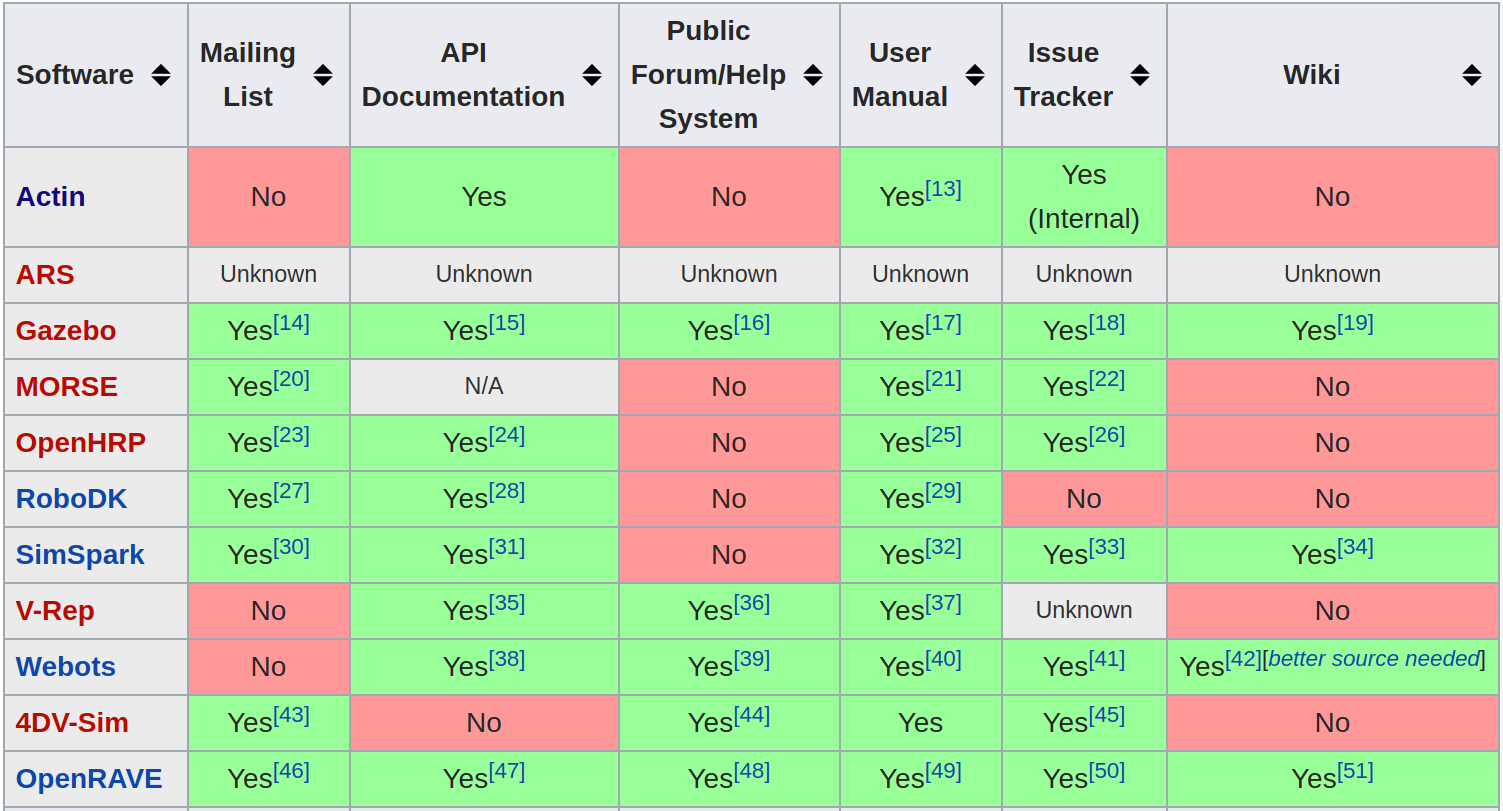
\includegraphics[width=.9\textwidth]{img/WikipTableRobSim.png}
  \caption{Types of support the different robot simulators provides\cite{wikiRobSim}}
  \label{fig:infra}
\end{figure}

With Gazebo you can place a 3D model of the robot arm in a 3D scenario where you can place different other objects and for example test out different object avoidance algorithms. Gazebo comes with a good physics engine which give good simulation of the inertia and gravity impacting the robot\cite{Gazebo}. This is important because these are the two effects which impact the robot most. This will hopefully make the transition between the simulated robot and the real robot less complicated. \\\\
It can be useful to know that Gazebo is a simulation tool simulates the real world with physics. RVIZ is just a visualization tool used for visualize the inputs you are sending it and does not do any simulation. 




%For simulation and visualization in ROS, Rviz and Gazebo are used. Gazebo is a simulation environment with a good physics engine which can be used to simulate and test different control algorithms. Rviz is just a visualization tool to visualize the robot configuration and is great to use along with control of actual hardware. 



%\begin{figure}[htbp]
%  \centering
%  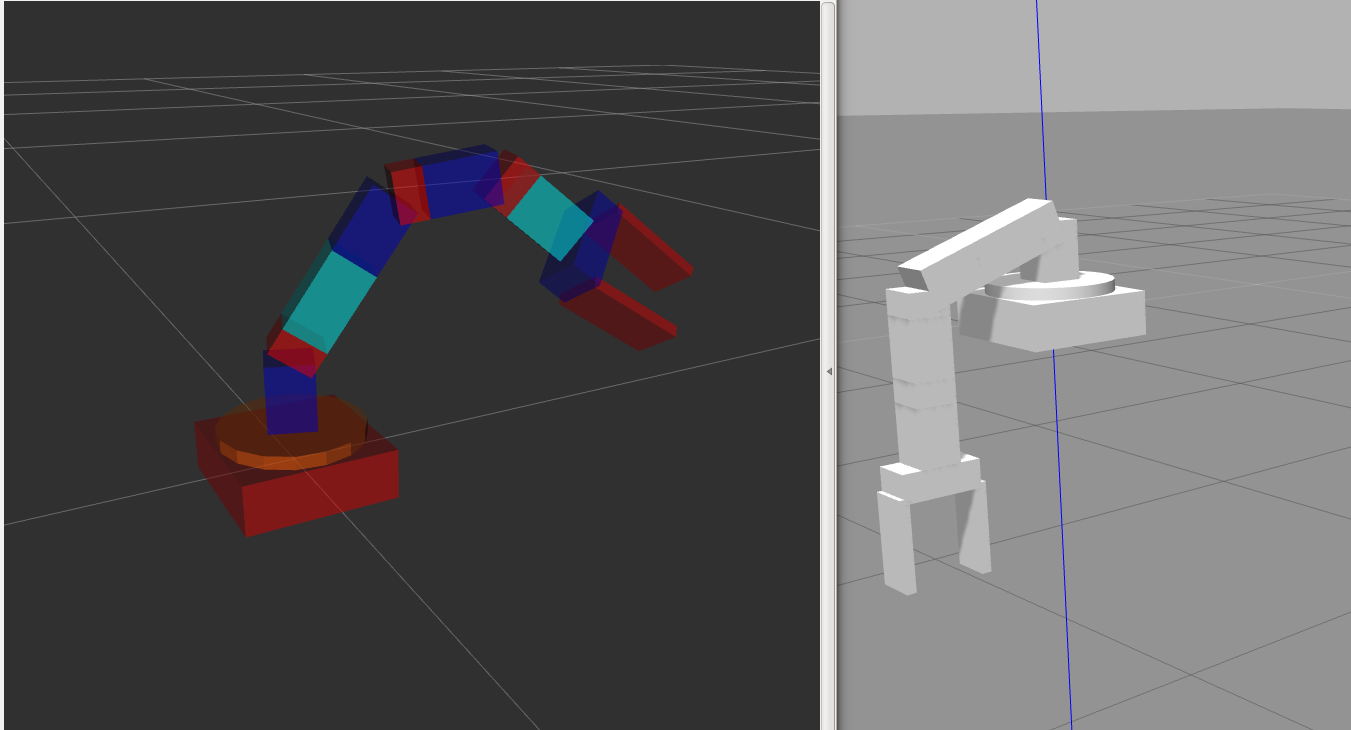
\includegraphics[width=.9\textwidth]{img/test.png}
%  \caption{Manipulators visualized in Rviz and Gazebo, respectively}
%  \label{fig:robot}
%\end{figure}


\section{File types}
All the code can be found at this GitHub repository: \href{https://github.com/Aarskog/robotarm}{\underline{https://github.com/Aarskog/robotarm}}\\

Now that the software to be used is found and installed the next step is to provide right tools to connect it together. There are three different types of files that are important when making the robot, spawning it and make it to accept inputs and broadcast its current joint states. 
\begin{itemize}
    \item URDF - Describes the 3D model of the robot
    \item YAML - Describes the joint controllers and its parameters
    \item launch - Describes what processes to start on launch.
\end{itemize}
A brief description of the files is given in the sections below.  If one want a more detailed description the following resources can be useful \cite{ROSWiki,GazeboURDF,XMLdoc,YAMLdoc}.

\subsection{Unified Robot Description Format (URDF)}\label{sec:basicURDF}
The code used in the URDF is XML code which means that the syntax is very easy to understand\cite{XMLdoc}. When building your robot there are two main components that is the base of the file. The first is the link element that describes a part of the robot. In \lstref{lst:example} a link element is presented. This element describes a cylinder where the length and radius is given and defines the measurements of the link. 


\begin{lstlisting}[language=xml,caption={URDF code example of a link element},label={lst:example}]
<link name="base_link">
    <visual>
        <geometry>
            <cylinder length="0.6" radius="0.2"/>
        </geometry>
    </visual>
</link>
\end{lstlisting}
The second important element is the joint element. When you have multiple links it is desirable to connect them together with joints. In \lstref{lst:jointexample} an example of a joint element is given. This gives the URDF parser information about how two links are connected. In this example \textit{link1} is the parent link of \textit{link2} the origin of the axes of rotation is given by the origin which is [0,0,1] which means that the origin of \textit{link2} is shifted 1 meter in the z direction relative to \textit{link2}. The joint type is revolute and it rotates about the z axis of the parent link. 

\begin{lstlisting}[language=xml,caption={URDF code example of a joint element},label={lst:jointexample}]
<joint name="joint_name" type="revolute">
    <parent link="link1"/>
    <child link="link2"/>
    <origin xyz="0 0 1"/>
    <axis xyz="0 0 1"/>
</joint>
\end{lstlisting}
This is the very basic for construction a object using URDF. A more detailed walkthrough is given when the method of construction of the robot is given in section \ref{sec:makingurdf}\cite{ROSWiki}.


\subsection{YAML-Yet Another Markup Language}
YAML is Unicode based data serialization language. It is useful for configuration files and internet messaging among many other things \cite{YAMLdoc}. In the project, the \textit{joints.yaml} file is the configuration file that states the torque controller properties for each joint. As per now a PID controller is used for each joint. This is based on a SISO system for the joints. The dynamic equations of the manipulator is in fact a complex nonlinear and multivariable system\cite{spong}.

\subsection{Launch files}
The launch files are used for starting up Gazebo,Rviz and the different nodes used for control and broadcasting joint states. It is also used to place the robot model into the simulation environment. The controller nodes are launched from \textit{control.launch} in the ROS package. 



























\section{Robotic manipulator description}
In \figref{fig:robotAH} a picture of the actual robot is given. It is a five degrees of freedom robotic arm. Five degrees of freedom means in this case that the robot arm has five joints that we can control. All of the joints of this robot manipulator are rotating joints\cite{Crustcrawler}. 

\begin{figure}[htbp]
  \centering
  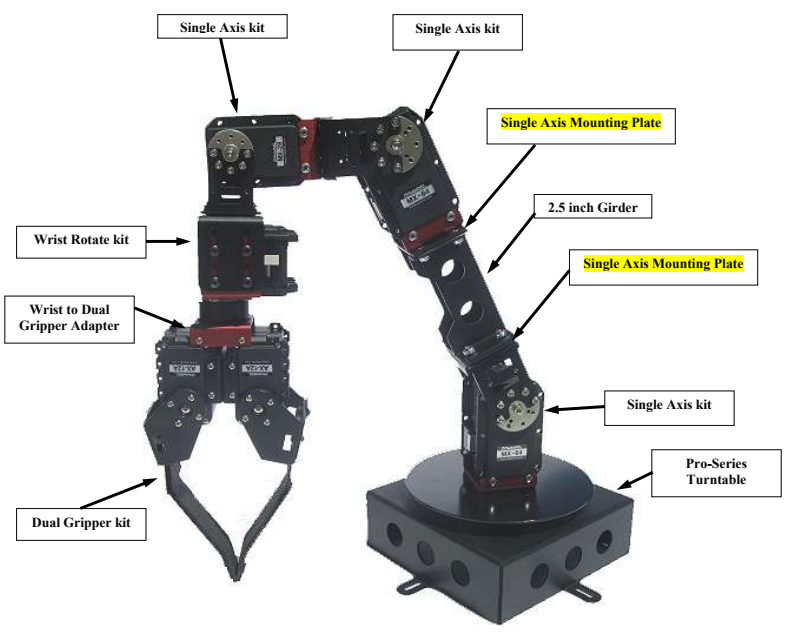
\includegraphics[width=.7\textwidth]{img/robotAH.png}
  \caption{Robot at hand}
  \label{fig:robotAH}
\end{figure}



The URDF includes mass and inertia as parameters which is possible to add a property of the joint. With this is mind the first to do is to find the mass of the different components that the robot at hand consists of. In \figref{fig:robotAH} for modelling and simulation the turntable base mass is not important to know since it is assumed that it is an unmoveable object that is stuck on the world frame. \\

\subsection{Dividing the robot into parts}
As briefly explained in section \ref{sec:basicURDF} the robot must be described as a series of links and joints. For the robot to be properly modelled with the URDF, it is desirable to find and classify the different parts of the robotic arm.\\\\
%In \tabref{table:partlist} the parts of the robot manipulator taken from the datasheet is listed\cite{Crustcrawler}.
The part list of the robot manipulator is seen in \tabref{table:partlist} taken from the datasheet \cite{Crustcrawler}. \tabref{table:partlist} is the initial list that was used as a base for constructing the robot. And in \figref{fig:utgangspunkt} the part names are set their respective places on the robot. 

\begin{table}[htbp]
\centering
\caption{Partlist of the relevant parts taken from the datasheet and web-page of the robot}
\label{table:partlist}
    \begin{tabular}{ l r}
        \toprule
        Partname  & Amount \\
        \midrule
        MX-28T Pro-Series Turntable & 1\\
        MX-64T Pro-Series Single Axis kits& 2\\
        AX Short Bracket(SSB-Short) & 3\\
        2.5 inch(6.35cm) Pro Series Girder & 1 \\
        MX-28T Pro-Series Single Axis kit & 1 \\
        MX-28T Pro-Series Wrist Rotate kit & 1\\
        Pro-Series Wrist to Dual Gripper Adapter & 1\\
        Dual gripper kit with two AX-12A Servos& 1\\
               \bottomrule
    \end{tabular}
\end{table}



\begin{figure}[htbp]
  \centering
  \includesvg[width=.9\textwidth]{img/utgangpunktURDF.svg}
  \caption{Robot sketch}
  \label{fig:utgangspunkt}
\end{figure}



\subsection{Finding mass and moments of inertia}
All the other weights above the turntable must be known. Unfortunately the datasheet does not give specific information about all of the parts. More of items were found in the webstore, but not all. The rest had to be guesstimated. For example the mass of circular plate which the rest of the arm stands on is not given explicitly. In \tabref{table:partmass} the different masses of the parts are presented.\\\\ 
\begin{table}[htbp]
\centering
\caption{Mass of parts}
\label{table:partmass}
    \begin{tabular}{l c r}
        \toprule
        Part  &  Weight(kg) & Estimated\\
        \midrule
        MX-28T Pro-Series Turntable Plate& 0.05 & yes\\
        MX-64T Pro-Series Single Axis kits& 0.126 & no\\
        AX Short Bracket (SSB-Short) & 0.01 & yes\\
        2.5 inch(6.35cm) Pro Series Girder & 0.0227 & no\\
        MX-28T Pro-Series Single Axis kit & 0.072 & no \\
        MX-28T Pro-Series Wrist Rotate kit & 0.127 & no\\
        Pro-Series Wrist to Dual Gripper Adapter & 0.126 & yes\\
        Dual gripper kit with two AX-12A Servos& 0.01 & yes\\
        \bottomrule
    \end{tabular}
\end{table}
The next thing that is necessary to find, is the moments of inertia of the links of the manipulator. As seen from \figref{fig:robotAH} the parts have different shapes and lengths so it can be a challenge to find the exact moments of inertia. A simplification is therefore needed. The simplification that is used is to model them as boxes with uniform weight distribution. To calculate the moment of inertia the width,length and height of the part are needed. To simplify the naming of the different parts the following names seen in \figref{fig:naming} are used.\\


\begin{figure}[htbp]
  \centering
  \includesvg[width=.9\textwidth]{img/utgangpunktURDFWithNaming.svg}
  \caption{Robot sketch with simplified names}
  \label{fig:naming}
\end{figure}

\begin{table}[htbp]
\centering
\caption{Measurements of parts}
\label{table:measurements}
    \begin{tabular}{l c c c r}
        \toprule
        Part  &  x - Width(meter) & y - Length(meter) & z - Height(meter)\\
        \midrule
        Base & 0.1143 & 0.1143 & 0.0381\\
        Turntable & 0.055(radius) & NA & 0.01\\
        Motor2345 & 0.0356 & 0.0355 & 0.0506 \\
        Bracket123 & 0.0356 & 0.0355 & 0.0206 \\
        Girder & 0.0356 & 0.0355 & 0.0635\\
        Adapter & 0.0356 & 0.0710 & 0.0253\\
        Left/right finger & 0.03568 & 0.0089 & 0.08\\
        \bottomrule
    \end{tabular}
\end{table}


The complete documentation on the different parts is not complete. This means that some of the lengths has to be guesstimated\cite{Crustcrawler}. In the simplified model (\figref{fig:naming}) there are only boxes except the turntable which is a small cylinder. For the boxes the following inertia matrix is used

\begin{align*}
    I = 
    \begin{bmatrix}
        I_{xx} & 0 & 0\\
        0 & I_{yy} & 0\\
        0 & 0 & I_{zz}
    \end{bmatrix}
\end{align*}
where
\begin{align*}
    I_{xx} &= \frac{1}{12}m(height^2+length^2)\\
    I_{yy} &= \frac{1}{12}m(height^2+width^2)\\
    I_{zz} &= \frac{1}{12}m(length^2+width^2)
\end{align*}
for the parts which are modelled as boxes and 
\begin{align*}
    I_{xx} &= \frac{1}{12}m(3r^2+height^2)\\
    I_{yy} &= \frac{1}{12}m(3r^2+height^2)\\
    I_{zz} &= \frac{1}{2}mr^2
\end{align*}
for the cylindrical turntable \cite{Dupac}. 

\begin{table}[htbp]
\centering
\caption{List of inertias. Base is left out because it is fixed to the world frame and it is not neceassary to calculate this inertia}
\label{table:inertia}
    \begin{tabular}{l c c r}
        \toprule
        Part  &  $I_{xx}$ & $I_{yy}$ & $I_{zz}$\\
        \midrule
        Turntable & $3.82\cdot10^{-5}$ &  $3.82\cdot10^{-5}$ &$2.27\cdot10^{-4}$\\
        Motor2345 & $4.01\cdot10^{-5}$  & $4.01\cdot10^{-5}$  & $2.65\cdot10^{-5}$ \\
        Bracket123 & $1.40\cdot10^{-6} $ & $1.40\cdot10^{-6} $ & $2.10\cdot10^{-6} $ \\
        Girder & $1.00\cdot10^{-5} $ & $1.00\cdot10^{-5} $ & $4.80\cdot10^{-6} $\\
        Adapter & $5.97\cdot10^{-5} $ & $2.00\cdot10^{-5} $ & $6.62\cdot10^{-5} $\\
        Left/right finger & $~0$ & $~0$ & $0$\\
        \bottomrule
    \end{tabular}
\end{table}
%The moments of inertia are very small, and axis of rotation needs to be checked. It is also unknown how the URDF reader uses the inertia and how much it is up to the user to do adjustments. When construction the robot it is built in sequence from the bottom and up by adding part by part. The parent link of the first part is the world frame.

\section{Constructing the robot using URDF}\label{sec:makingurdf}
Now everything need to make the URDF file is found and the calculations needed is done. The first object to be made is the base. Again a more detailed walk through can be found at \cite{ROSWiki,GazeboURDF}\\
\begin{lstlisting}[language=xml,caption={Base},label={lst:base}]
<link name="base_link">
    <visual>
        <geometry>
            <box size ="${basex} ${basey} ${basez}"/>
        </geometry>
        <origin xyz="0 0 0" rpy="0 0 0"/>
    </visual>
    <inertial>
        <origin xyz="0 0 0" rpy="0 0 0"/>
        <mass value="2"/>
        <inertia ixx="1" ixy="0" ixz="0" iyy="1" iyz="0" izz="1" />
    </inertial>
    <collision>
        <origin xyz ="0 0 0"/>
        <geometry>
            <box size ="${basex} ${basey} ${basez}"/>
        </geometry>
    </collision>
</link>
\end{lstlisting}
In \lstref{lst:base} the URDF code is presented. The declaration can be divided into three parts: Visual, inertal and collision. The different parts are self explanatory. The values for the moment of inertia and the mass is set to one since the base is fixed to the world which means that it will not move and the values chosen for it does not matter. The next object to be constructed is the turntable plate which will rotate on top of the base. How the turntable is made can be seen in the attached code, but it is the same method used in \lstref{lst:base}, but with the values given in \tabref{table:partmass}, \tabref{table:measurements} and \tabref{table:inertia}. To connect the two link objects a joint element has to be made. The code used for this is seen in \lstref{lst:jointBTT}.

\begin{lstlisting}[language=xml,caption={joint between base and turntable},label={lst:jointBTT}]
<joint name="base_to_turntable" type="continuous">
  <parent link="base_link"/>
  <child link="turntable"/>
  <origin xyz="0 0 ${(basez+turntable_height)/2}$"/>
  <axis xyz ="0 0 1"/>
</joint>
\end{lstlisting}
One thing to notice when making the joint element, is to place the turntable at the right position relative to the base and get it to rotate the way it is supposed to rotate. When placing the origin of the joint, it is adjusted relative of the origin of the parent link. Moving the joint origin will move the origin of the child link. Therefore the joint origin is set to half of the sum of the height of the two links. This will place the turntable on top of the base. The axis is the axis of rotation which is the z-axis. This was the joint for the twisting joint. The other twisting joint is modelled the same way. For the rotational joints(joints 2,3 and 4) the axis of rotation is about the x-axis relative to the its parent link. \\\\
After all the links and joints are placed, the model needs to be spawned in Gazebo. To do this, launch files are used. To start Gazebo with an empty world the following code shown in \lstref{lst:empty} is used
\begin{lstlisting}[language=xml,caption={Start Gazebo with empty world},label={lst:empty}]
<include file="$(find gazebo_ros)$/launch/empty_world.launch">
  <arg name="paused" value="false"/>
  <arg name="use_sim_time" value="true"/>
  <arg name="gui" value="true"/>
  <arg name="headless" value="false"/>
  <arg name="debug" value="false"/>
</include>
\end{lstlisting}
the last two elements are given in \lstref{lst:l2} where the first line is a script that needs to be run since macros\footnote{Macros is something that is used in URDF to simplify the coding by allowing to make templates and declare variables etc.} is used. The second line creates the node that will spawn the robot into Gazebo. 
\begin{lstlisting}[caption={Spawn robot model in Gazebo},label={lst:l2},language=xml]
  <param name="robot_description" command="$(find xacro)/xacro.py $(arg model)" />

  <node name="urdf_spawner" pkg="gazebo_ros" type="spawn_model"
        args="-z 0.01905 -pause -urdf -model robot -param robot_description" respawn="false" output="screen" />
\end{lstlisting}
In \figref{fig:RG} the result is presented. As one can see in \figref{fig:flaccid} the robot arm will just fall to the ground when the simulation is started. This is of course expected since no joint control has been added yet. In the next chapter the method of doing control will be presented. 

\begin{figure}[htbp]
  \centering
  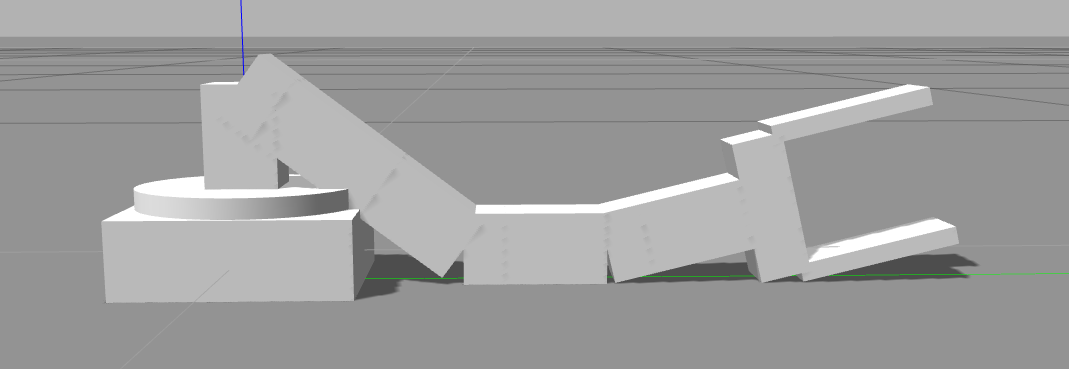
\includegraphics[width=.9\textwidth]{img/gazeG.png}
  \caption{Screenshot of the robot in Gazebo with no joint control}
  \label{fig:flaccid}
\end{figure}

\begin{figure*}[htbp]
    \centering
    \begin{subfigure}[htbp]{0.45\textwidth}
        \centering
        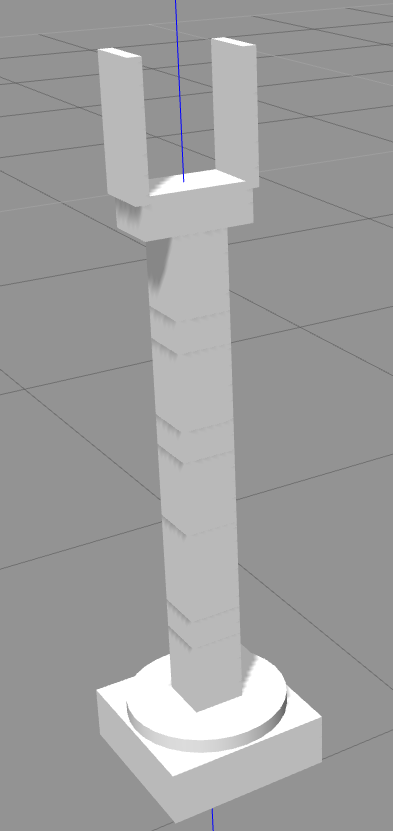
\includegraphics[width = 1\linewidth]{img/robotGazUP.png}
        \caption{The robot arm visualized in Gazebo}
        \label{fig:robgaz}
    \end{subfigure}
    ~ 
    \begin{subfigure}[htbp]{0.45\textwidth}
        \centering
        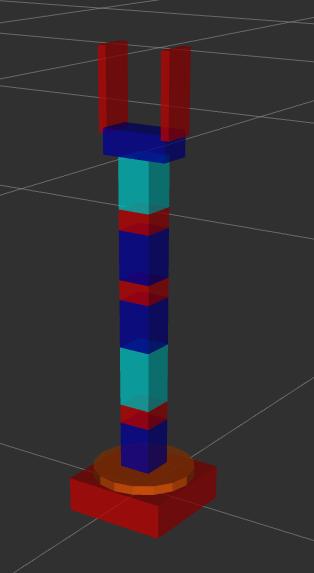
\includegraphics[width = 1\linewidth, height = 0.705\textheight]{img/rvizRass.png}
        \caption{The robot arm visualized in RViz}
        \label{fig:robviz}
    \end{subfigure}
    \caption{The robot arm visualized in Gazebo and RViz}
    \label{fig:RG}
\end{figure*}
\chapter{Kinematics}
As we already know the robot can be represented as a kinematic chain of links and connected by revolute joints. In this chapter the forward kinematics for this robotic manipulator is calculated and a method for solving the inverse kinematics is proposed. 

\section{Forward Kinematics}
The forward kinematics states the relationship between the end effector and the individual joints. Or as \cite{Siciliano} says it: The motion of the structure is obtained by composition of the elementary motions of each link with respect to the previous one. An easy way to get the forward kinematics is to use the Denavit-Hartenberg(DH) convention. \cite{spong} states that each homogeneous transformation $A_i$ is represented as a product of four basic transformations: 

$$
A_i = \text{Rot}_{z,\theta_i}\text{Trans}_{z,d_i}\text{Trans}_{x,a_i}\text{Rot}_{x,\alpha_i}=
    \begin{bmatrix}
        c_{\theta_i} & -s_{\theta_i}c_{\alpha_i} & s_{\theta_i}s_{\alpha_i} & a_ic_{\theta_i}\\
        s_{\theta_i} & c_{\theta_i}c_{\alpha_i} & -c_{\theta_i}s_{\alpha_i} & a_is_{\theta_i}\\
        0 & s_{\alpha_i} & c_{\alpha_i} &d_i\\
        0 & 0 & 0 & 1
    \end{bmatrix}
$$

where $c_{\theta_i} = \cos{(\theta_i)}$ and $s_{\theta_i} = \sin{(\theta_i)}$, and the same for $\alpha$. $A_i$ is a transformation matrix which states the transformation between link number $i$ and link number $i-1$. This means that it is possilbe to get the transformation from the robot base to the end effector by multiplying each transformation matrix:
\begin{align*}
    T^i_j = A_{i+1}A_{i+2}...A_j, \quad i<j
\end{align*}
 $T^i_j$ states the transformation between each link and it has the form
 \begin{align*}
      T^i_j = 
      \begin{bmatrix}
          R^i_j & o^i_j\\
          0&1
      \end{bmatrix}, \quad i<j
 \end{align*}
 where $R^i_j = R^i_{i+1}R...R^{j-1}_j$ which is the orientation of $o_jx_jy_jz_j$ relative to $o_ix_iy_iz_i$. $o^i_j$ is the coordinate vector which can be written as $o^i_j = o^i_{j-1}+R^{i}_{j-1}o^{j-1}_j$. This is useful when finding the Jacobian of the robot and to verify that the end effector is at the wanted position and has the wanted orientation in the Cartesian world frame. When finding the DH-parameters they have to satisfy the two following properties (\cite{spong}).
 \begin{itemize}
     \item The axis $x_n$ is perpendicular to the axis $z_{n-1}$
     \item The axis $x_n$ intersects the axis $z_{n-1}$
 \end{itemize}

In \figref{fig:dhf} the different axis are set with respect to the DH properties stated above. 

\begin{figure}[htbp]
  \centering
  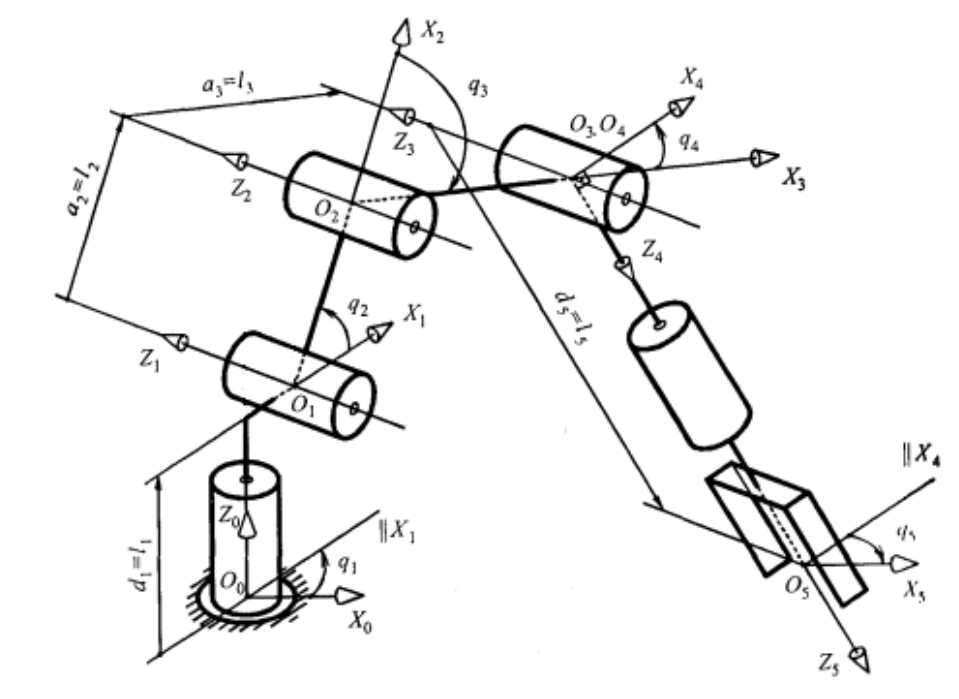
\includegraphics[width=.9\textwidth]{img/DHconv.png}
  \caption{Kinematic scheme of the manipulator. Source \cite{Kinematics}}
  \label{fig:dhf}
\end{figure}

By looking at \figref{fig:dhf} the following DH parameters are found:
\begin{center}
    \begin{tabular}{|c|c|c|c|c|}
         \hline
         Link & $a_i$ & $\alpha_i$ & $d_i$ & $\theta_i$ \\ \hline
         1 & 0 & $-\frac{\pi}{2}$ & $d_1$ & $q_1$ \\
         2 & $a_2$ & 0 & 0 & $q_2$ \\ 
         3 & $a_3$ & 0 & 0 & $q_3$\\
         4 & 0 & $\frac{\pi}{2}$ & 0 & $q_4$\\
         5 & 0 & 0 & $d_5$ & $q_5$\\
         \hline
    \end{tabular}
\end{center}

% d_1 = 0.0506
% a_2 = 0.0506 + 0.0206 + 0.0635 = 0.1347
% a_3 = 0.0506 + 0.0206 = 0.0712
% d_5 = 0.0506 + 0.0206 + 0.0253 + 0.08 = 0.1765

where $d_1 = 0.0506$, $a_2 = 0.1347$, $a_3 = 0.0712$ and $d_5 = 0.1765$ for the model. The real values need to be measured properly since the data sheet of the robot is insufficient and this is just guesstimated values. 
Now it is possible to calculate $A_i$ for each link: 
\begin{align*}
A_1 &= \begin{bmatrix} 
            c_1 & 0 & -s_1 & 0\\
            s_1 & 0 & c_1 & 0\\
            0 & -1 & 0 & d_1\\
            0 & 0 & 0 & 1
        \end{bmatrix},
A_2 = \begin{bmatrix} 
            c_2 & -s_2 & 0 & a_2c_2\\
            s_2 & c_2 & 0 & a_2s_2\\
            0 & 0 & 1 & 0\\
            0 & 0 & 0 & 1
        \end{bmatrix},
A_3 = \begin{bmatrix} 
            c_3 & -s_3 & 0 & a_3c_3\\
            s_3 & c_3 & 0 & a_3s_3\\
            0 & 0 & 1 & 0\\
            0 & 0 & 0 & 1
        \end{bmatrix}\\
A_4 &= \begin{bmatrix} 
            c_4 & 0 & s_4 & 0\\
            s_4 & 0 & -s_4 & 0\\
            0 & 1 & 0 & 0\\
            0 & 0 & 0 & 1
        \end{bmatrix},
A_5 = \begin{bmatrix} 
            c_5 & -s_5 & 0 & 0\\
            s_5 & c_5 & 0 & 0\\
            0 & 0 & 1 & d_5 \\
            0 & 0 & 0 & 1
        \end{bmatrix}
\end{align*}
 and then calculate $T_i^0$:
\begin{subequations}
    \begin{align}
        T_1^0 &= A_1 =
        \begin{bmatrix}\label{eq:T1}
            c_1 & 0 & -s_1 & 0\\
            s_1 & 0 & c_1 & 0\\
            0 & -1 & 0 & d_1\\
            0 & 0 & 0 & 1
        \end{bmatrix}\\
        T_2^0 &= A_1A_2 =
        \begin{bmatrix}\label{eq:T2}
            c_1c_2 & -c_1s_2 & -s_1 & a_2c_1c_2\\
            s_1c_2 & -s_1s_2 & c_1 & a_2s_1c_2\\
            -s_2 & -c_2 & 0 & d_1 - a_2s_2\\
            0 & 0 & 0 & 1
        \end{bmatrix}\\
        T_3^0 &= A_1A_2A_3=
        \begin{bmatrix}\label{eq:T3}
            c_{23}c_1 & -c_1s_{23} & -s_1 & c_1(a_3c_{23} + a_2c_2)\\
            c_{23}s_1 & -s_1s_{23} & c_1 & s_1(a_3c_{23} + a_2c_2)\\
            -s_{23} & -c_{23} & 0 & d_1 - a_3s_{23}-a_2s_2\\
            0 & 0 & 0 & 1
        \end{bmatrix}\\
        T_4^0 &= A_1A_2A_3A_4=
        \begin{bmatrix}\label{eq:T4}
            c_1c_{234} & -s_1 & c_1s_{234} & c_1(a_3c_{23} + a_2c_2)\\
            s_1c_{234} & c_1 & s_1s_{234} & s_1(a_3c_{23} + a_2c_2)\\
            -s_{234} & 0 & c_{234} & d_1 - a_3s_{23} - a_2s_2\\
            0 & 0 & 0 & 1
        \end{bmatrix}\\
        \begin{split}
            T_5^0 &= A_1A_2A_3A_4A_5\\ &=
            \begin{bmatrix}\label{eq:T5}
                c_1c_{234}c_5 - s_1s5 & -s_1c_5 - c_1c_{234}s_5 & c_1s_{234} & c_1(a_3c_{23} + a_2c_2 + d_5s_{234})\\
                s_1c_{234}c_5 + c_1s_5 & c_1c_5 - s_1c_{234}s_5 & s_1s_{234} & s_1(a_3c_{23} + a_2c_2 + d_5s_{234})\\
                -s_{234}c_5 & s_{234}s_5 & c_{234} & d_1 - a_3s_{23} - a_2s_2 + d_5c_{234}\\
                0 & 0 & 0 & 1
            \end{bmatrix}
        \end{split}
     \end{align}
\end{subequations}
where $s_{ijk} = \sin{(q_i + q_j + q_k)}$ and the same for $c_{ijk}$. 
%The $T_i^0$ matrix can be sectioned into
%\begin{align*}
 %T_i^0 = 
  %  \begin{bmatrix}
   %     \bm{R}(\bm{q}) & \bm{p}(\bm{q})\\
    %    \bm{0}^T & 1
    %\end{bmatrix}    
%\end{align*}

%-----------------------------------------------------------------------------------------
\begin{comment}
\begin{align*}
    T^0_5 &= A_1A_2A_3A_4A_5\\
    &= 
    \begin{bmatrix}
        c_1c_{234}c_5 + s_1s_5 & -c_1c_{234}s_5+s_1c_5 & -c_1s_{234} & c_1(-d_5s_{234} + a_3c_{23} + a_2c_2)\\
        c_1c_{234}c_5 - s_1s_5 & -s_1c_{234}s_5-c_1c_5 & -s_1s_{234} & s_1(-d_5s_{234} + a_3c_{23} + a_2c_2) \\
        -s_{234}c_5 & s_{234}s_5 & -c_{234} &d_1 - a_2s_2 - a_3s_{23} - d_5c_{234}\\
        0 & 0 & 0 & 1\\
    \end{bmatrix}\\
    &=
    \begin{bmatrix}
        \bm{R}(\bm{q}) & \bm{p}(\bm{q})\\
        \bm{0}^T & 1
    \end{bmatrix}
\end{align*}
\end{comment}
%-----------------------------------------------------------------------------------------

\subsection{Direct kinematics}
(Just a smaller representation of the forward kinematics)

\subsection{Jacobian}
As we already know the forward kinematics can be written as:
\begin{align*}
    T(q) = 
    \begin{bmatrix}
        R(q) & p(q)\\
        0 & 1
    \end{bmatrix}
\end{align*}
we want to express the linear velocity $\dot{p}$ and angular velocity $\omega$ as a function of the joint velocities $\dot{q}$. In \cite{Siciliano} the relations is stated as:

\begin{equation}
    \begin{aligned}\label{eq:velo}
        \dot{p} &= J_P(q)\dot{q}\\
        \omega&= J_O(q)\dot{q}
    \end{aligned}
\end{equation}

where $J_O$ with dimensions (3 $\times$ n) is the relation between the joint velocities $\dot{q}$ and the end-effector linear velocity $\dot{p}$, and the (3 $\times$ n) matrix $J_O$ is the relation between the joint velocities $\dot{q}$ and the end-effector angular velocity $\omega$. \eqref{eq:velo} can be written as

\begin{align*}
    v_e = 
    \begin{bmatrix}
        \dot{p} \\ \omega
    \end{bmatrix}
    = J(q)\dot{q}
\end{align*}
where
\begin{align*}
    J = 
    \begin{bmatrix}
        J_P \\ J_O
    \end{bmatrix}
\end{align*}

which is the matrix that \cite{Siciliano} calls the geometric Jacobian. The elements of 
$$
J = 
\begin{bmatrix}
    j_{P1} & & j_{Pn}\\
    &...&\\
    j_{O1} & & j_{On}
\end{bmatrix}
$$
can be calculated in the following way:
\begin{align*}
    \begin{bmatrix}
        j_{Pi}\\j_{Oi}
    \end{bmatrix}
    =
    \begin{cases}
        \begin{bmatrix} z_{i-1}\\ 0 \end{bmatrix} & \text{for a prismatic joint}\\
        \begin{bmatrix} z_{i-1} \times (p_e-p_{i-1}) \\ z_{i-1} \end{bmatrix} & \text{for a revolute joint}
    \end{cases}
\end{align*}

Since our manipulator only has revolute joints, the geometric Jacobian becomes

\begin{align*}
    J(q) = 
    \begin{bmatrix}
        z_0 \times (p_5-p_0) & 
        z_1 \times (p_5-p_1) & 
        z_2 \times (p_5-p_2) & 
        z_3 \times (p_5-p_3) & 
        z_4 \times (p_5-p_4) \\
        z_0 &
        z_1 &
        z_2 &
        z_3 &
        z_4
    \end{bmatrix}
\end{align*}
From when the forward kinematics were calculated each position vector $p_i$ can be directly obtained from the equations \eqref{eq:T1} - \eqref{eq:T5}:



\begin{align*}
    p_0 = \begin{bmatrix} 0 \\ 0 \\ 0 \end{bmatrix}    \quad
    p_1 = \begin{bmatrix} 0 \\ 0 \\ d_1\end{bmatrix}    \quad
    p_2 = \begin{bmatrix} a_2c_1c_2\\ a_2s_1c_2\\ d_1 - a_2s_2\end{bmatrix}   \quad 
    p_3 = \begin{bmatrix} c_1(a_3c_{23} + a_2c_2) \\ s_1(a_3c_{23} + a_2c_2) \\ d_1 - a_3s_{23}-a_2s_2 \end{bmatrix}  \\  
    p_4 = \begin{bmatrix} c_1(a_3c_{23} + a_2c_2) \\ s_1(a_3c_{23} + a_2c_2) \\ d_1 - a_3s_{23}-a_2s_2\end{bmatrix}  \quad  
    p_5 = \begin{bmatrix} c_1(a_3c_{23} + a_2c_2 + d_5s_{234}) \\ s_1(a_3c_{23} + a_2c_2 + d_5s_{234}) \\ d_1 - a_3s_{23} - a_2s_2 + d_5c_{234} \end{bmatrix}    
\end{align*}

The next step is to find $z_{i-1}$. \cite{Siciliano} states that $z_{i-1}$ is given by the third column of the rotation matrix $R_{i-1}^0$. $R_{i-1}^0$ is already given in $T_i^0$, By looking at \eqref{eq:T1} - \eqref{eq:T5} the following values of $z_{i-1}$ is given:
\begin{align*}
    z_0 &= \begin{bmatrix}0\\0\\1\end{bmatrix},
    z_1 = \begin{bmatrix}-s_1\\c_1\\0\end{bmatrix},
    z_2 = \begin{bmatrix}-s_1\\c_1\\0\end{bmatrix},
    z_3 = \begin{bmatrix}-s_1\\c_1\\0\end{bmatrix},
    z_4 = \begin{bmatrix}c_1s_{234}\\s_1s_{234}\\c_{234}\end{bmatrix}
\end{align*}

now we got everything needed to compute the geometric Jacobian and the result is presented below.


\begin{align*}
    J(q) &= \\
    &\begin{bmatrix}
        -s_1(a_3c_{23} + a_2c_{2} + d_5s_{234}) & 
        -c_1(a_3s_{23} + a_2s_{2} - d_5c_{234}) & 
        -c_1(a_3s_{23} - d_5c_{234})            & 
        c_1d_5c_{234}                           & 
        0\\
        c_1(a_3c_{23} + a_2c_{2} + d_5s_{234})  & 
        -s_1(a_3s_{23} + a_2s_{2} - d_5c_{234}) & 
        -s_1(a_3s_{23} - d_5c_{234})            & 
        s_1d_5c_{234}                           & 
        0\\
        0                                       &
        -a_3c_{23}- a_2c_2 - d_5s_{234}         &
        -a_3c_{23} - d_5s_{234}                 &
        -d_5s_{234}                             &
        0\\
        0                                       &
        -s_1                                    &
        -s_1                                    &
        -s_1                                    &
        c_1s_{234}\\
        0                                       &
        c_1&
        c_1&
        c_1&
        s_1s_{234}\\
        1& 0 & 0 & 0 & c_{234}
    \end{bmatrix}
\end{align*}
which has the full rank of $5$. 

















\section{Inverse Kinematics}

As we already know, the forward kinematics establishes the relationship between the joint variables and the position and orientation of the end effector. The problem of inverse kinematics is to find the joint variables when the position and orientation of the end effector is given. This is wanted because the wanted position or trajectory is given in the Cartesian world frame. Unfortunately the inverse kinematics problem is not as easy and straight forward as the forward kinematics problem. \cite{Siciliano} lists up several reasons the inverse kinematics problem is so much more complex:
\begin{itemize}
    \item The equations to solve are in general nonlinear, and thus it is not always possible to find a closed-form solution.
    \item Multiple solutions may exist.
    \item Infinite solutions may exist, e.g., in the case of a kinematically redundant manipulator.
    \item There might be no admissible solutions, in view of the manipulator kinematic structure.
\end{itemize}
There are different methods of solving the inverse kinematics problem. One way to solve it is to solve it algebraically. Ideally you want a function that has the orientation and position as input and then gives the respective joint angles. In our case where we have a 5 DOF robot arm the equations becomes too large and too difficult to solve, \cite{spong}. By looking at the equation $T_5^0=H$ where $T_5^0$ is given in \eqref{eq:T5} and $H$ is the desired transformation matrix of the end effector. It shows us that it gives a complex set of equations to solve. Another thing that must be consideres is that not all joints in our system can rotate 360 degrees either so if a solution is to be found it may not work because of the limitations of the robot manipulator. \\

It is also possible to use a geometric approach where the thought is to find the joint angels by projecting the manipulator onto the previous plane[\cite{spong}] and solve it using trigonometry. Both \cite{spong} and \cite{Siciliano} uses simple manipulators and special cases where simplifications can be made. \\

After some research in making a inverse kinematics solver from the bottom and up with constraints and everything, it was found that this will not yield satisfactory results. The choice was therefore to use an already existing solver. Many solvers did not support a 5 DOF robot manipulator, but after some research the choice fell upon a MATLAB robotics toolbox(https://se.mathworks.com/help/robotics/). The toolbox makes a great interface with ROS which makes it easy to create subscribers and listeners here as well. A useful part is that it is possible to include the URDF file where MATLAB creates a robot object and represent the robot manipulator as something called rigid body tree. In other words it is just the way MATLAB parses the URDF file. In \figref{fig:showRovs} the MATLAB function $show(robot)$ is used and you can see the visualization of the robot. This can be used to check solutions and it can be though as a simpler version of RViz. The right finger is shifted to the center to use it as a inverse kinematics reference point. 

\begin{figure}[htbp]
  \centering
  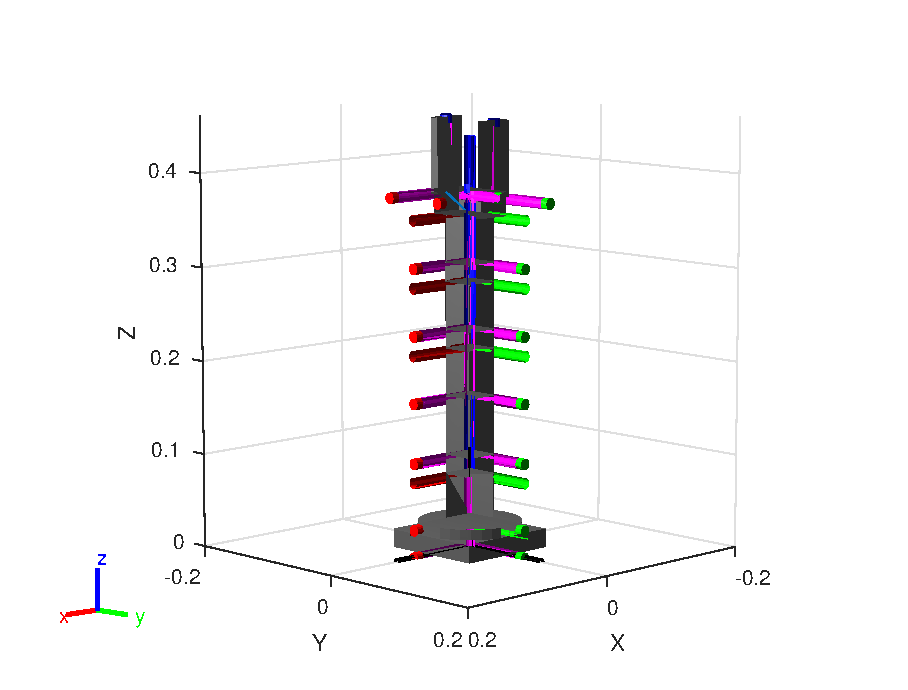
\includegraphics[width=.9\textwidth]{img/showRobs.eps}
  \caption{MATLAB visualization of the robot using URDF}
  \label{fig:showRovs}
\end{figure}

In \lstref{lst:robotinit} seen below the robot object is created. The inverse kinematics solver object is also created. The initial solver of the inverse kinematics problem is the \textit{Broyden–Fletcher–Goldfarb–Shanno} (BFGS) algorithm which is an iterative, gradient-based optimization method that start with an initial guess to minimize a cost function \cite{MatlabRobTool}. The other solving algorith is the \textit{Levenberg-Marquardt} algorithm which is not as good if you only have the home configuration of the robot, but it is faster. So if you are to follow a path it could be a good choice to use \textit{Levenberg-Marquardt}. 

\begin{lstlisting}[caption={MATLAB code of creating a invrerse kinematics},label={lst:robotinit},language=Matlab]
robot = importrobot('robot.urdf');
ik = robotics.GeneralizedInverseKinematics('RigidBodyTree',robot);
ik.ConstraintInputs={'joint','position','orientation'};
ik.SolverParameters.SolutionTolerance = 0.00001;
ik.SolverParameters.GradientTolerance = 0.000001;
ik.SolverParameters.MaxTime = 0.1;
ik.SolverParameters.AllowRandomRestart = 0;
\end{lstlisting}

The \lstref{lst:gik} show an example of finding the inverse kinematics. Here we want the end effector denoted 'right finger' which was moved to the center for a reference point, to reach the position $pd$ with the orientation $od$. It is also wanted to have some constraints such that the solution is at a feasible configuration which is seen at line 6 to 10. Again the datasheets does not state the operational limits of the joints 2,3 and 4, so the bounds has been guessed. The bounds of the twisting joints 1 and 5 are set to $\pm \pi$ to avoid solutions past these bounds. 

\begin{lstlisting}[caption={MATLAB code of creating a inverse kinematics},label={lst:gik},language=Matlab]
posTgt = robotics.PositionTarget('right_finger');
posTgt.TargetPosition = pd';
orTgt = robotics.OrientationTarget('right_finger');
orTgt.TargetOrientation = eul2quat(od');
jointConst = robotics.JointPositionBounds(robot);
jointConst.Bounds = [-pi,pi;
                -3*pi/4,3*pi/4
                -3*pi/4,3*pi/4
                -3*pi/4,3*pi/4
                -pi,pi];
initialguess = robot.homeConfiguration;
[configSoln,solInfo] = ik(initialguess,jointConst,posTgt,orTgt);
qd = [configSoln(:).JointPosition]';
\end{lstlisting}














































\begin{comment}


\cite{Siciliano} states that one can use the Jacobian of the system to calculate the inverse kinematics:

\begin{align}\label{eq:algo}
\dot{\bm{e}} = \dot{\bm{x}}_d - \bm{J}_A(\bm{q})\dot{\bm{q}}
\end{align}

In \figref{fig:inverseAlgo} the inverse kinematics algorithm is stated. From the figure one can see that 
$$
\dot{\bm{q}} = \bm{J}_A^{-1}(\bm{q})(\dot{\bm{x}}_d + \bm{K}e)
$$
where K is a positive definite diagonal matrix which makes the resulting system \eqref{eq:algo} into the linear system
\begin{align*}
    \dot{\bm{e}} + \bm{K}e = \bm{0}
\end{align*}


\begin{figure}[htbp]
  \centering
  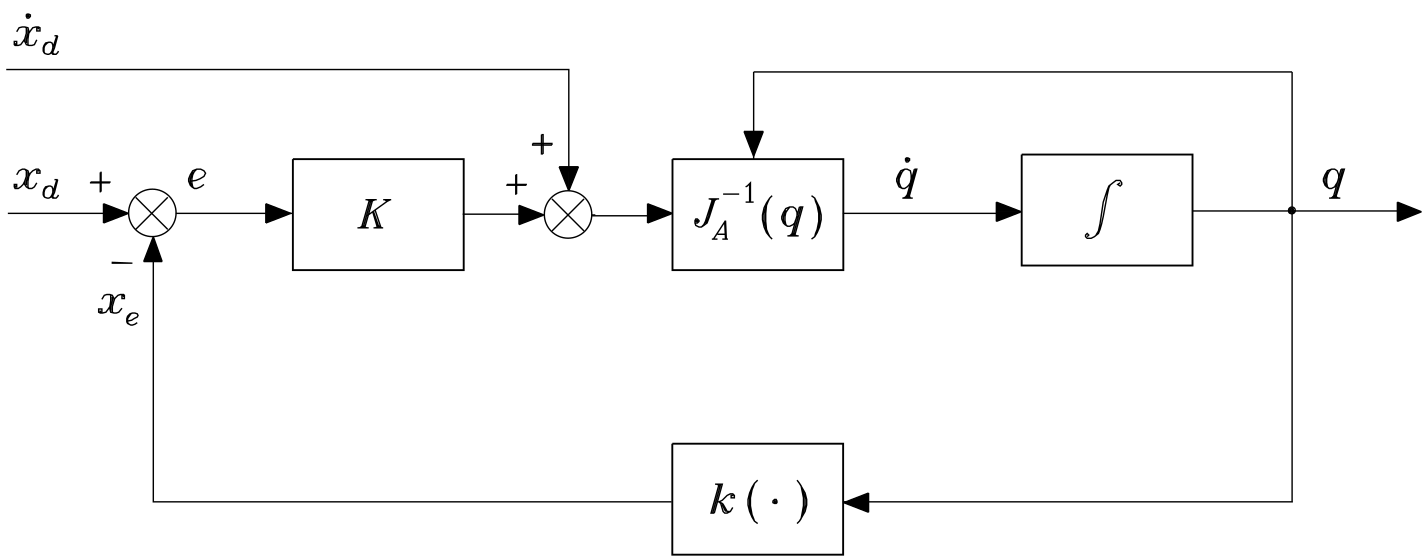
\includegraphics[width=.9\textwidth]{img/inverseKin.png}
  \caption{Inverse kinematics algotihm with Jacobian inverse. Source \cite{Siciliano}.}
  \label{fig:inverseAlgo}
\end{figure}

\subsubsection*{Analytical Jacobian}
To use the algorithm in \figref{fig:inverseAlgo} the analytical Jacobian is needed. In \cite{Siciliano} the following relationship is given
\begin{align*}
    \bm{J}_A =
    \begin{bmatrix}
        \bm{I} & \bm{0}\\ 0 & \bm{T}^{-1}(\bm{\phi_e})
    \end{bmatrix}
    \bm{J}(\bm{q})
\end{align*}

where $\bm{\phi_e} = [\phi,\theta,\psi]^T$ is the orientation of the end-effector frame relative to the base frame given by the Euler angles ZYZ. From \eqref{eq:T5} the rotation matrix from the base frame to end-effector is
\begin{align*}
    \bm{R}_5^0 &= 
    \begin{bmatrix}
        r_{11} & r_{12} & r_{13}\\
        r_{21} & r_{22} & r_{23}\\
        r_{31} & r_{32} & r_{33}
    \end{bmatrix}
    =
    \begin{bmatrix}
        c_1c_{234}c_5 - s_1s_5 & -s_1c_5 - c_1c_{234}s_5 & c_1s_{234}\\
        s_1c_{234}c_5 + c_1s_5 & c_1c_5 - s_1c_{234}s_5 & s_1s_{234}\\
        -s_{234}c_5 & s_{234}s_5 & c_{234} 
    \end{bmatrix}
\end{align*}

The ZYZ Euler angles are then


\begin{align*}
    \phi &= atan2(r_{21},r_{11}) = atan2(s_1c_{234}c_5 + c_1s_5,c_1c_{234}c_5 - s_1s_5)\\
    \theta &= atan2\left(-r_{31},-\sqrt{r_{32}^2+r_{33}^2}\right) = atan2\left(s_{234}c_5,-\sqrt{s_{234}s_5^2+c_{234}^2}\right)\\
    \psi &= atan2(r_{32},r_{33}) = atan2(s_{234}s_5,c_{234})
\end{align*}

The angular velocity $\bm{\omega}_e$ and $\bm{T}(\bm{\alpha})$ is given as

\begin{align*}
    \bm{\omega} = 
    \begin{bmatrix}
        0 & -s_\phi & c_\phi s_\theta\\
        0 & c_\phi & s_\phi s_\theta\\
        1 & 0 & c_\theta
    \end{bmatrix}
    \begin{bmatrix}
        \dot{\phi}\\\dot{\theta}\\\dot{\psi}
    \end{bmatrix}
    =
    \bm{T}(\bm{\phi}_e)\dot{\bm{\phi}}_e
\end{align*}
The determinant of $\bm{T}$ is $-s_\theta$ which means that one cannot invert for $\theta = 0,\pi$. This singularity is also the singularity of the geometric Jacobian. 








\section{Motion planning}




If the desired position is $p$ and the desired orientation is $R$. Then in \cite{Kinematics}, the inverse kinematics are given as: 

\begin{align*}
    q_1 &= \tan^{-1}{\left(\frac{p_y}{p_x}\right)}\\
    q_2 &= atan2\left( a(a_2+a_3c_3) - ba_3s_3, aa_3s_3 + b(a_2+a_3c_3) \right)\\%atan2
    q_3 &= \cos^{-1}{\left(\frac{a^2+b^2-a^2_2-a^2_3}{2a_2a_3}\right)}\\
    q_4 &= q_{234} - q_2 - q_3\\
    q_5 &= c_{234}q_1-2atan(R_{21},R_{11})
\end{align*}

where $a = d_1 - d_5c_{234}-p_z$, $b = p_xc_1 + p_ys_1+d_5s_{234}$ and $-\frac{\pi}{2}<q_1 < \frac{\pi}{2}$. $q_{234} = atan2\left(\frac{p_x}{c_1p_x+s_1p_y})\right)$


\end{comment}
\chapter{Control}

Now that a functioning simulation environment is created and a inverse kinematics solver is created it is time to connect these to and create a controller to steer the robot manipulator. The initial thought is a multivariable control on top on single joint control. The multivariable control is done in Matlab, but it can be done in Python as well, but since the inverse kinematics problem is solved in MATLAB it is easiest to do the control in MATLAB. The multivariable control will use the joint positions and joint velocities to compute the desired joint torques which is sent to joint PID controllers which is handled by using ROS control package. The first thing to do is therefore to create the individual joint PID controllers. 
To create these controllers two new files are needed. A new launch file must be created. It is possible to just append the launch file, but to make everything more understandable and if the package is to be used on the real robot it is easier to make a new launch file that can be included in other launch files. The task of the control.launch file is to spawn a node which includes all of the five controllers. In \lstref{lst:launchControl} one can see the the code to spawn the controllers. It consists of two statements. The first is loading the parameters of the controllers from the YAML file. Then with the parameters loaded, a node is created and it makes the joint controller services that the wanted joint torques can be published to. 
\begin{lstlisting}[language=xml,caption={Spawns the controller node},label={lst:launchControl}]
<rosparam file="$(find five_dof_robotarm)/config/joints.yaml" command="load"/>

  <node name="controller_spawner" pkg="controller_manager" type="spawner" respawn="false"
	output="screen" ns="/five_dof_robotarm" args="joint_state_controller
    base_to_turntable_controller
    second_joint_controller
    third_joint_controller
    fourth_joint_controller
    fifth_joint_controller"/>
\end{lstlisting}
Below in \lstref{lst:matlabPubl} one can see how the publishers that will publish the desired joint torques calculated by the controller. 
\begin{lstlisting}[language=Matlab,caption={MATLAB code for creating the publishers.},label={lst:matlabPubl}]
pub1 = rospublisher('/five_dof_robotarm/base_to_turntable_controller/command','std_msgs/Float64');
pub2 = rospublisher('/five_dof_robotarm/second_joint_controller/command','std_msgs/Float64');
pub3 = rospublisher('/five_dof_robotarm/third_joint_controller/command','std_msgs/Float64');
pub4 = rospublisher('/five_dof_robotarm/fourth_joint_controller/command','std_msgs/Float64');
pub5 = rospublisher('/five_dof_robotarm/fifth_joint_controller/command','std_msgs/Float64');
\end{lstlisting}
%Pythoncode
\begin{comment}
\begin{lstlisting}[language=python,caption={Python code for creating the publishers.},label={lst:pythonPubl}]
#Define publishers for each joint position controller commands.
pub1 = rospy.Publisher('/five_dof_robotarm/first_joint_controller/command', Float64, queue_size=10)
pub2 = rospy.Publisher('/five_dof_robotarm/second_joint_controller/command', Float64, queue_size=10)
pub3 = rospy.Publisher('/five_dof_robotarm/third_joint_controller/command', Float64, queue_size=10)
pub4 = rospy.Publisher('/five_dof_robotarm/fourth_joint_controller/command', Float64, queue_size=10)
pub5 = rospy.Publisher('/five_dof_robotarm/fifth_joint_controller/command', Float64, queue_size=10)
\end{lstlisting}
\end{comment}


And how to publish the wanted torques is seen below in \lstref{lst:matlabPubs}. Here $u$ is the vector of the controller output. During the project it was also wanted to do the same in Matlab and the initial thought is the same and can be viewed in the appendix. 

\begin{lstlisting}[language=Matlab,caption={MATLAB code for publish wanted joint torques},label={lst:matlabPubs}]
    send(pub1,u(1))
    send(pub2,u(2))
    send(pub3,u(3))
    send(pub4,u(4))
    send(pub5,u(5))
\end{lstlisting}

\begin{comment}
\begin{lstlisting}[language=python,caption={Python code for publish wanted torques},label={lst:pythonPubs}]
pub1.publish(u[0,0])
pub2.publish(u[1,0])
pub3.publish(u[2,0])
pub4.publish(u[3,0])
pub5.publish(u[4,0])
\end{lstlisting}
\end{comment}


Another important functionallity to do control is to get the feedback from Gazebo with joint position and joint velocities. To do this a subscriber is needed. The subscriber can thought of as the opposite as the publisher. Instead of publishing values to a service, we instead want to listen to a service. 


\section{Control}

\subsection{PD controller with gravity compensation}

The controller that is going to be used is a simple PD controller with gravity compensation derived by \cite{spong}:
$$
    u=K_p\tilde{q} - K_d\dot{q} +g(q)
$$
 where $\tilde{q} = q_d - q$ and 
 \begin{align}\label{eq:gravity}
 g(q) = \frac{\partial P}{\partial q_k}
 \end{align}
 where the total potential energy for a n-link robot is $P = \sum^n_{i=1}P_i$. Where $P_i$ is the potential energy for each individual link. For this specific manipulator the center of mass is assumed in the geometric center of each link. In \cite{Siciliano} this controller is proven by using Lyapunov direct method to be globally asymptotically stable(GAS) as long as $K_d$ and $K_p$ is positive definite. It is important to keep in mind that if the online computing of $g(q)$ is not perfect, the statement of GAS does not hold. Based on the assumptions made, the controller can not guarantee GAS. 
 
 \subsection{Deriving the gravitational effect}
 The robot at hand starts and ends with twisting joints and only the three joints in the middle is rotational joints. This means that the potential energy is only dependent on $q_2$,$q_3$ and $q_4$ which makes calculating the potential energy a bit a easier. Because of this, the potential energy can be calculated by using a 2D sketch as shown in \figref{draw:pot-rob}.

\begin{figure}[htbp]
    \centering
    

%Thank you http://www.texample.net/tikz/examples/three-link-annotated/

\usetikzlibrary{patterns}

\newcommand{\nvar}[2]{%
    \newlength{#1}
    \setlength{#1}{#2}
}

% Define a few constants for drawing
\nvar{\dg}{0.3cm}
\def\dw{0.25}\def\dh{0.5}
\nvar{\ddx}{1.5cm}

% Define commands for links, joints and such
\def\link{\draw [double distance=1.5mm, very thick] (0,0)--}
\def\joint{%
    \filldraw [fill=white] (0,0) circle (5pt);
    \fill[black] circle (2pt);
}
\def\grip{%
    \draw[ultra thick](0cm,\dg)--(0cm,-\dg);
    \fill (0cm, 0.5\dg)+(0cm,1.5pt) -- +(0.6\dg,0cm) -- +(0pt,-1.5pt);
    \fill (0cm, -0.5\dg)+(0cm,1.5pt) -- +(0.6\dg,0cm) -- +(0pt,-1.5pt);
}
\def\robotbase{%
    \draw[rounded corners=8pt] (-\dw,-\dh)-- (-\dw, 0) --
        (0,\dh)--(\dw,0)--(\dw,-\dh);
    \draw (-0.5,-\dh)-- (0.5,-\dh);
    \fill[pattern=north east lines] (-0.5,-1) rectangle (0.5,-\dh);
}

% Draw an angle annotation
% Input:
%   #1 Angle
%   #2 Label
% Example:
%   \angann{30}{$\theta_1$}
\newcommand{\angann}[2]{%
    \begin{scope}[red]
    \draw [dashed, red] (0,0) -- (0pt,1.2\ddx);
    \draw [dashed, red] (0,0) -- (1.2\ddx,0pt);
    \draw [->, shorten >=3.5pt] ((0,\ddx) arc (90:#1:\ddx);
    % Unfortunately automatic node placement on an arc is not supported yet.
    % We therefore have to compute an appropriate coordinate ourselves.
    \node at (#1*2+2:\ddx-8pt) {#2};
    \end{scope}
}

% Draw line annotation
% Input:
%   #1 Line offset (optional)
%   #2 Line angle
%   #3 Line length
%   #5 Line label
% Example:
%   \lineann[1]{30}{2}{$L_1$}
\newcommand{\lineann}[4][0.5]{%
    \begin{scope}[rotate=#2, blue,inner sep=2pt]
        \draw[dashed, blue!40] (0,0) -- +(0,#1)
            node [coordinate, near end] (a) {};
        \draw[dashed, blue!40] (#3,0) -- +(0,#1)
            node [coordinate, near end] (b) {};
        \draw[|<->|] (a) -- node[fill=white] {#4} (b);
    \end{scope}
}

% Define the kinematic parameters of the three link manipulator.
\def\thetaone{30}
\def\Lone{2}
\def\thetatwo{30}
\def\Ltwo{1}
\def\thetathree{40}
\def\Lthree{1}


\begin{tikzpicture}
    %\robotbase
    \angann{\thetaone}{$q_2$}
    \lineann[-1]{\thetaone}{\Lone}{$L_2$}
    \link(\thetaone:\Lone);
    \joint
    \begin{scope}[shift=(\thetaone:\Lone), rotate=\thetaone]
        \angann{\thetatwo}{$q_3$}
        \lineann[-1.5]{\thetatwo}{\Ltwo}{$L_3$}
        \link(\thetatwo:\Ltwo);
        \joint
        \begin{scope}[shift=(\thetatwo:\Ltwo), rotate=\thetatwo]
            \angann{\thetathree}{$q_4$}
            \lineann[-1]{\thetathree}{\Lthree}{$L_4$}
            \draw [dashed, red,rotate=\thetathree] (0,0) -- (1.2\ddx,0pt);
            \link(\thetathree:\Lthree);
            \joint
            \begin{scope}[shift=(\thetathree:\Lthree), rotate=\thetathree]
                %\grip
            \end{scope}
        \end{scope}
    \end{scope}
\end{tikzpicture}

    \caption{Sketch of the robot the three middle joints of the robot}
    \label{draw:pot-rob}
\end{figure}
     
In \eqref{eq:potE} the potential energy is calculated for each link in the robot. 
 \begin{align}
    \begin{split}\label{eq:potE}
        P_1 &= m_1g\frac{L_1}{2}
        \\
        P_2 &= m_2g\left(L_1 + \frac{L_2}{2}\cos{(q_2)}\right)
        \\
        P_3 &= m_3g\left(L_1 +  L_2 \cos{(q_2)} + \frac{L_3}{2}\cos{(q_2 + q_3)} \right)
        \\
        P_4 &= m_4g\left(L_1 +  L_2 \cos{(q_2)} + L_3\cos{(q_2 + q_3)} + \frac{L_4}{2}\cos{(q_2+q_3+q_4)} \right)
        \\
        P_5 &=m_5g\left(L_1 +  L_2 \cos{(q_2)} + L_3\cos{(q_2 + q_3)} + \left(L_4 + \frac{L_5}{2} \right)\cos{(q_2+q_3+q_4)} \right)
        \\
        P &= P_1 + P_2 + P_3 + P_4 + P_5
    \end{split}   
 \end{align}    


 Where $L_4$ is the part up to the rotational joint. $L_5$ and $m_5$ is the rotational joint and the gripper together.  \\
 
 And then, to calculate individual gravity components equation \eqref{eq:gravity} is used on \eqref{eq:potE}:

 \begin{align*}
    g_1 &= 0
    \\
    g_2 &= \frac{\partial P}{\partial q_2} = 
    m_2g\frac{L_2}{2}\sin{(q_2)}+
    m_3g\left( L_2 \sin{(q_2)} + \frac{L_3}{2}\sin{(q_2+q_3)} \right)\\&+
    m_4g\left( L_2 \sin{(q_2)} + L_3\sin{(q_2 + q_3)} + \frac{L_4}{2}\sin{(q_2+q_3+q_4)} \right)\\&+
    m_5g\left( L_2 \sin{(q_2)} + L_3\sin{(q_2 + q_3)} + \left(L_4 + \frac{L_5}{2} \right)\sin{(q_2+q_3+q_4)} \right)
    \\
    g_3 &= \frac{\partial P}{\partial q_3} =
    m_3g\frac{L_3}{2}\sin{(q_2+q_3)} +
    m_4g\left( L_3\sin{(q_2 + q_3)} + \frac{L_4}{2}\sin{(q_2+q_3+q_4)} \right)\\&+
    m_5g\left(  L_3\sin{(q_2 + q_3)} + \left(L_4 + \frac{L_5}{2} \right)\sin{(q_2+q_3+q_4)} \right)
    \\
    g_4 &=\frac{\partial P}{\partial q_4} = 
    m_4g\frac{L_4}{2}\sin{(q_2+q_3+q_4)}+
    m_5g\left(L_4 + \frac{L_5}{2} \right)\sin{(q_2+q_3+q_4)}
    \\
    g_5 &= \frac{\partial P}{\partial q_5} = 0
    \\
    g(q) &= [g_1,g_2,g_3,g_4,g_5]^T
 \end{align*}
This is the gravity components that each joint will \textit{feel} from the other links and by adding this to a PD controller it will compensate for this disturbance. 

\section{Test of controller}
Now that a controller is in place it is time to test it. The first thing to test is the gravity compensation. One way to view the results is to watch the robot it is in a stationary state. The only input that are sent into the individual joint torque controllers should be the data computed only by the gravity compensation part. Some random desired joint angles is chosen and the following results can be viewed in \tabref{table:gravity}.\\\\
\begin{table}[htbp]
\centering
\caption{Test results of the precision of the gravity compensation}
\label{table:gravity}
    \begin{tabular}{l c c r}
        \toprule
        Joint  &  $g_i$ & $u_i$ & $u_i-g_i$\\
        \midrule
        1 & 0 & 0 & 0\\
        2 & -0.7720  & -0.7760  & -0.0040 \\
        3 &-0.4226 & -0.4191 & 0.0035 \\
        4 & -0.1870 &-0.1871 & -0.0001\\
        5 & 0 & 0 & 0\\
        \bottomrule
    \end{tabular}
\end{table}
One can see that the results are good. There is some error which means that the end effector will not be completely at its desired position. The biggest error is in the second joint and for this configuration $0.0022 rad = 0.1261 deg$\\\\
Now that we know that the gravity compensation is working we can start to test the controller. The gain matrices $K_p$ and $K_d$ are implemented as positive definite diagonal matrices.\\\\
\def\picsSiz{1.08}
\begin{figure*}[htbp]
    \centering
    \begin{subfigure}[htbp]{0.45\textwidth}
        \centering
        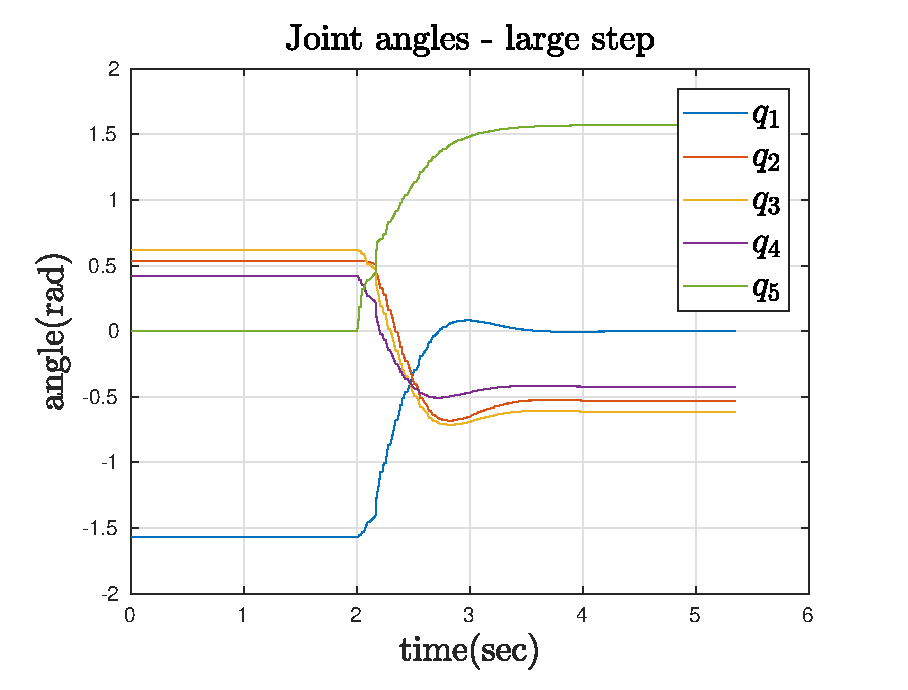
\includegraphics[width = \picsSiz\linewidth]{img/LSq.eps}
        \caption{ }
        \label{fig:LSq}
    \end{subfigure}
    ~ 
    \begin{subfigure}[htbp]{0.45\textwidth}
        \centering
        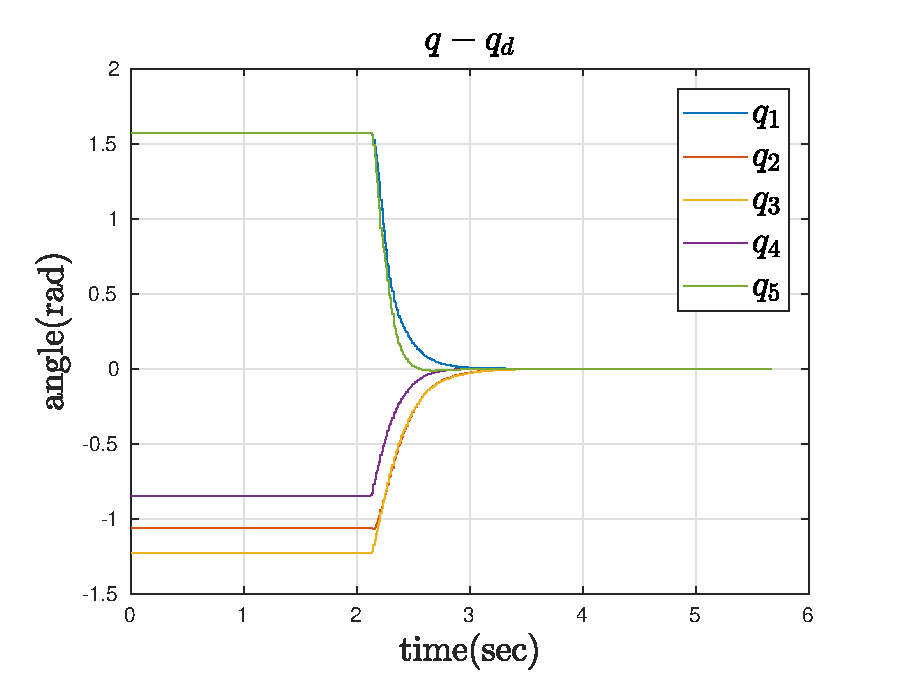
\includegraphics[width = \picsSiz\linewidth]{img/LSerror.eps}
        \caption{ }
    \end{subfigure}
    ~
    \centering
    \begin{subfigure}[htbp]{0.45\textwidth}
        \centering
        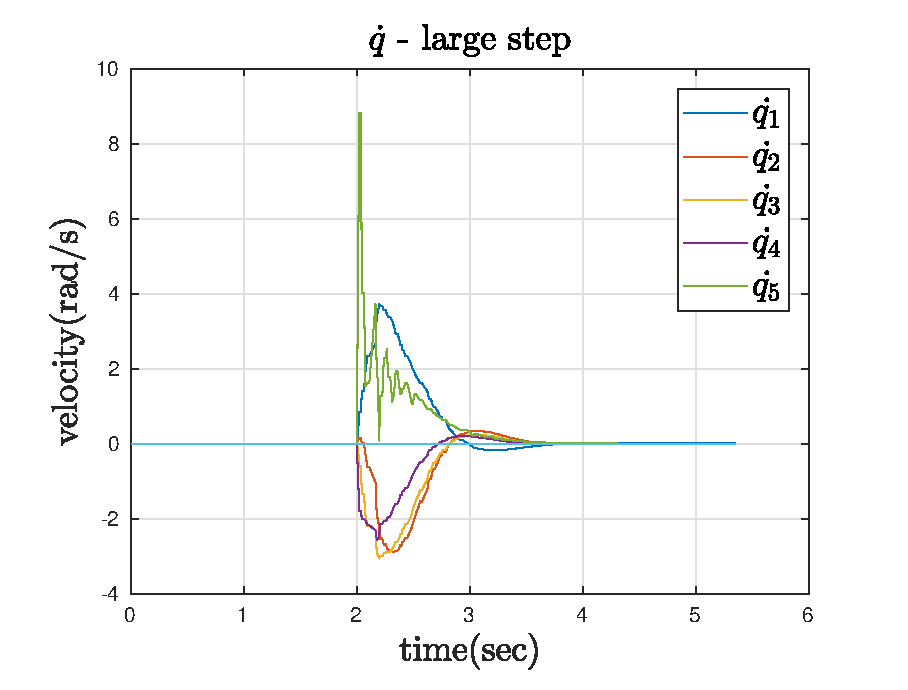
\includegraphics[width = \picsSiz\linewidth]{img/LSqdot.eps}
        \caption{ }
    \end{subfigure}
    ~ 
    \begin{subfigure}[htbp]{0.45\textwidth}
        \centering
        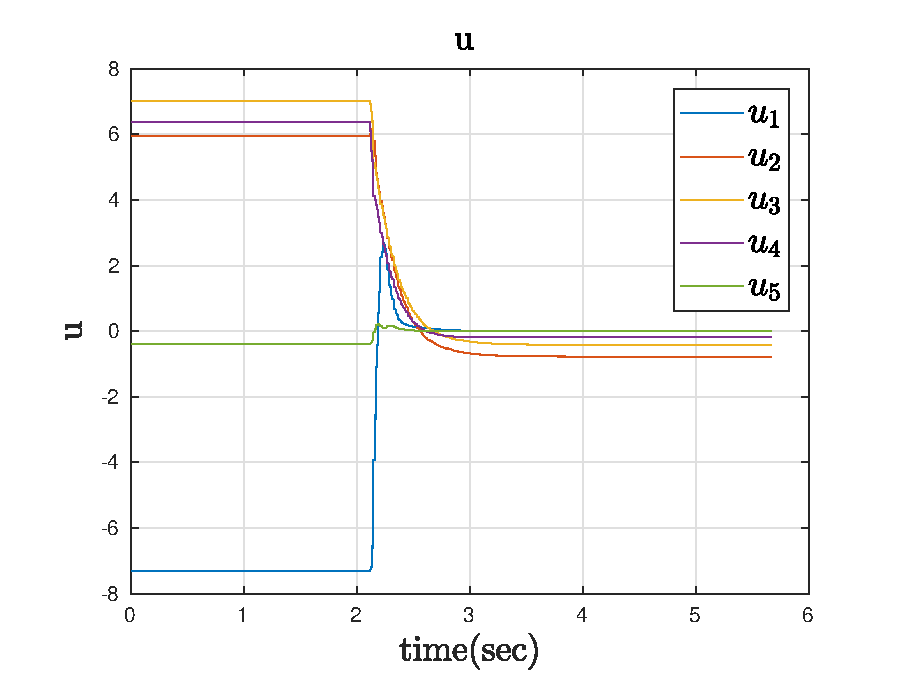
\includegraphics[width = \picsSiz\linewidth]{img/LSu.eps}
        \caption{ }
    \end{subfigure}
    ~
    \begin{subfigure}[htbp]{0.45\textwidth}
        \centering
        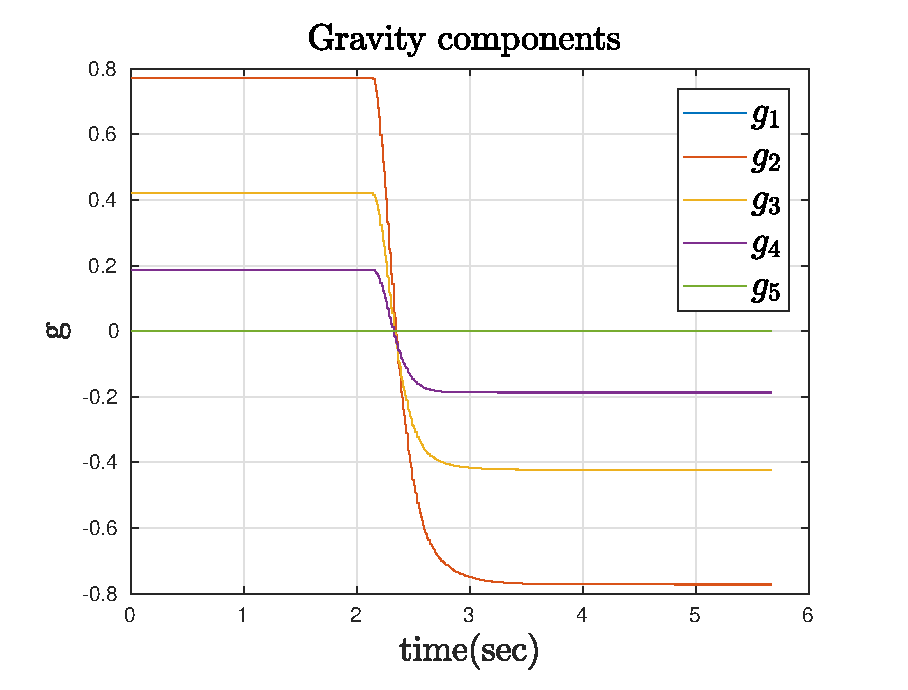
\includegraphics[width = \picsSiz\linewidth]{img/LSgrav.eps}
        \caption{ }
    \end{subfigure}
    \caption{Different plots of recorded data when a large step in desired joint angles is introduced}
    \label{fig:LS}
\end{figure*}
In \figref{fig:LS} data is plotted from a random configuration to a kind of inverse position such that every joint get to move. The step is rather large and because the intention of the robot arm is to do set point tracking some overshoot is therefore accepted for this case.  One thing that could be better is the joint velocity of last joint which seems a bit unstable. Additional tuning to try to avoid the bad input and joint velocity of the fifth joint results in slow convergence of the joint angle. Since the moments of inertia is very low and Gazebo handles low inertia very bad, this effect is assumed to be because of this and the when implementing this on the real robot it is expected that this effect will not be a problem. From \figref{fig:LSq} one can see $q_5$ converges rather smooth and the gains will be used for further testing. It may be worth to mention that when doing set point tracking the steps are not be this large and the gains can be altered for better performance.  \\\\






\section{Motion planning}



The main objective is to follow a path so it is desirable to test the controller for a path as well. The \figref{fig:pathTS} shows how each joint manages to follow the desired path. It is easy to see that we have a delay from the input to the output. This path is only time dependent so it changes without respect to if the robot arm has managed to get the desired position or not.\\
\def\picsSiz{1.08}
\begin{figure*}[htbp]
    \centering
    \begin{subfigure}[htbp]{0.45\textwidth}
        \centering
        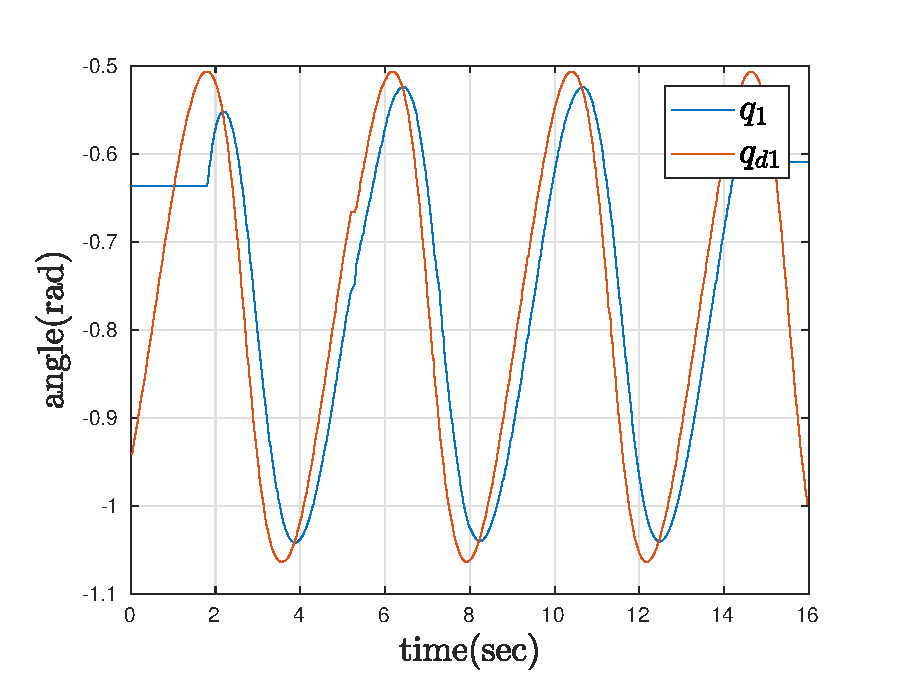
\includegraphics[width = \picsSiz\linewidth]{img/pathF1.eps}
        \caption{ }
    \end{subfigure}
    ~ 
    \begin{subfigure}[htbp]{0.45\textwidth}
        \centering
        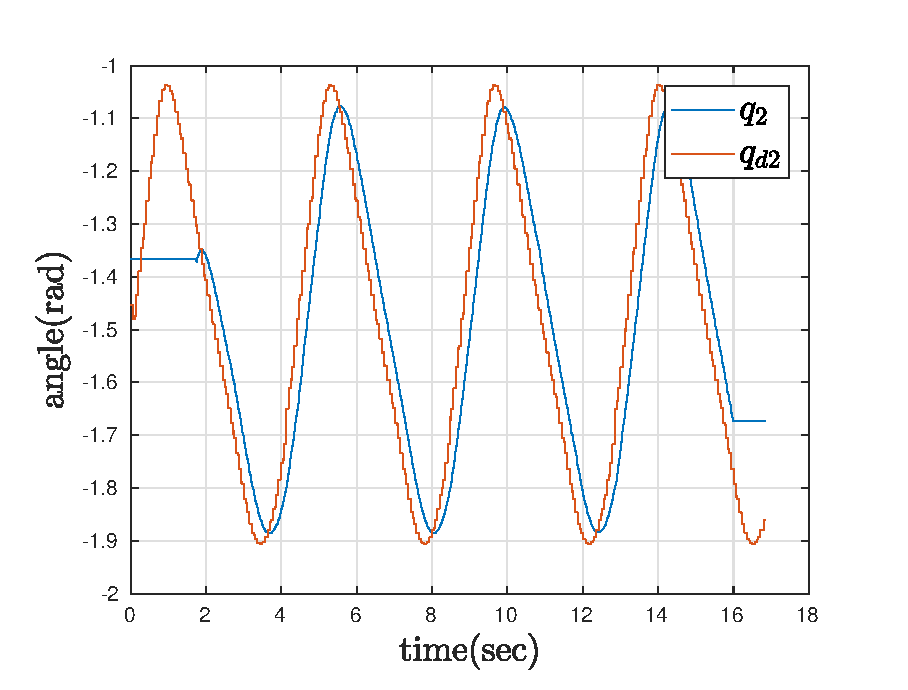
\includegraphics[width = \picsSiz\linewidth]{img/pathF2.eps}
        \caption{ }
    \end{subfigure}
    ~
    \centering
    \begin{subfigure}[htbp]{0.45\textwidth}
        \centering
        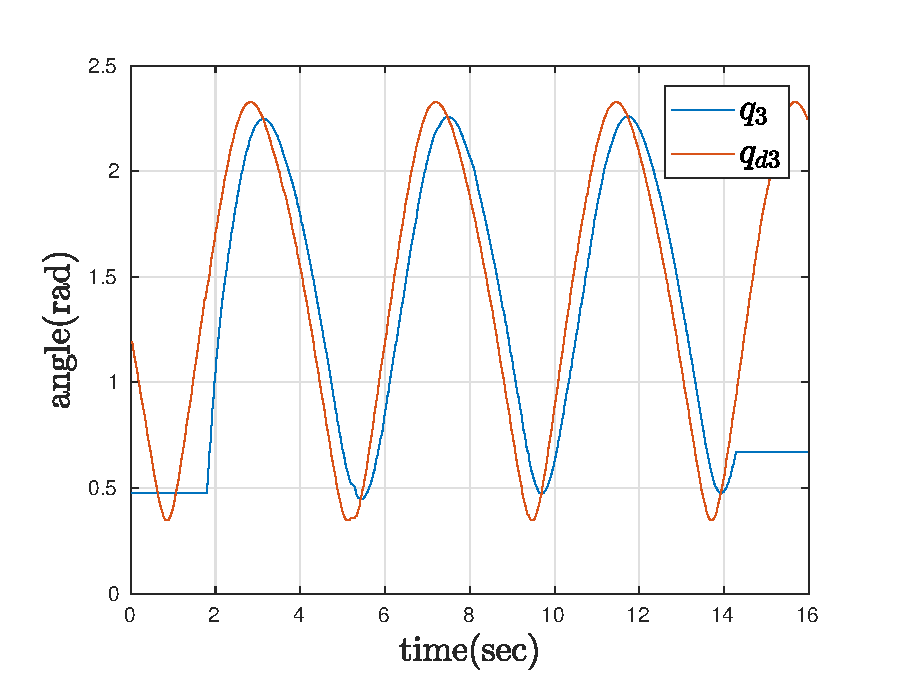
\includegraphics[width = \picsSiz\linewidth]{img/pathF3.eps}
        \caption{ }
    \end{subfigure}
    ~ 
    \begin{subfigure}[htbp]{0.45\textwidth}
        \centering
        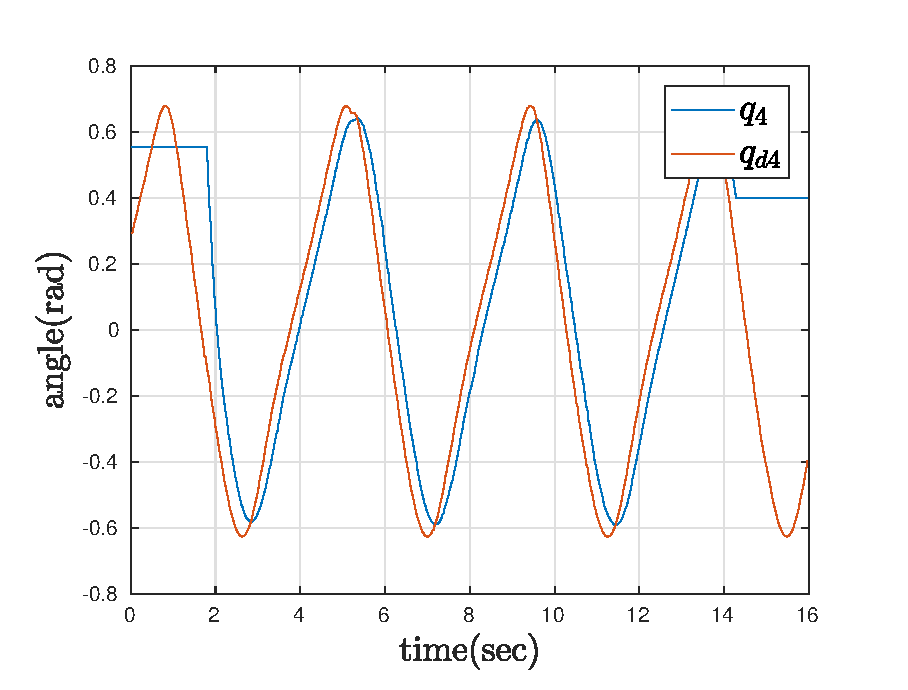
\includegraphics[width = \picsSiz\linewidth]{img/pathF4.eps}
        \caption{ }
    \end{subfigure}
    ~
    \begin{subfigure}[htbp]{0.45\textwidth}
        \centering
        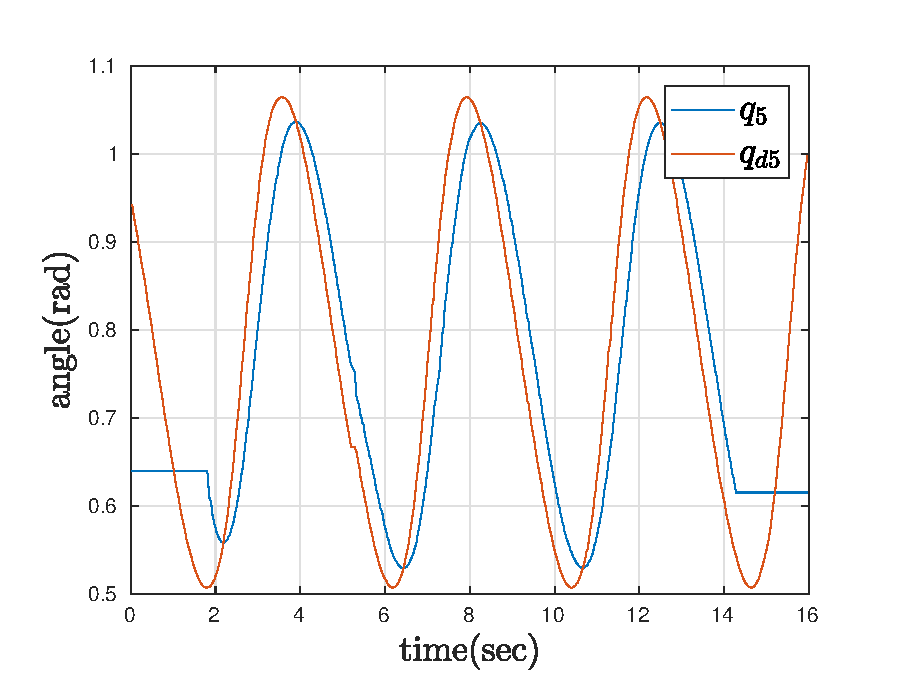
\includegraphics[width = \picsSiz\linewidth]{img/pathF5.eps}
        \caption{ }
    \end{subfigure}
    \caption{Path following}
    \label{fig:pathTS}
\end{figure*}
Since the results in \figref{fig:pathTS} is not so satisfactory a simple kind of feedforward was implemented. Since the path is calculated offline the informatioin about the next set points is used. The difference between desired state and current state has been $\tilde{q} = q_{d_i}-q$, but the new $\tilde{q}$ is now rewritten into 
\begin{align*}
    \tilde{q} = q_{d_ii}-q + \frac{q_{d_{i+1}}-q }{2}+\frac{q_{d_{i+2}}-q }{2}
\end{align*}
The results are given in \figref{fig:pathTSff}. It easy to see that the results is much better. It must be taken into consideration that $q_{d_i}$ is dependent on time and by introducing the two next set points the time shift becomes less apparent. If the next desired position is based on error(i.e. go to next point when you are close enough) instead of time based, the approach may be different. These results are of course given by a random path with only set points given and not desired joint velocity. A real motion planning algorithm should be used. This is just for showing the results. this means that a trajectory planner algorithm should be made. 



\def\picsSiz{1.08}
\begin{figure*}[htbp]
    \centering
    \begin{subfigure}[htbp]{0.45\textwidth}
        \centering
        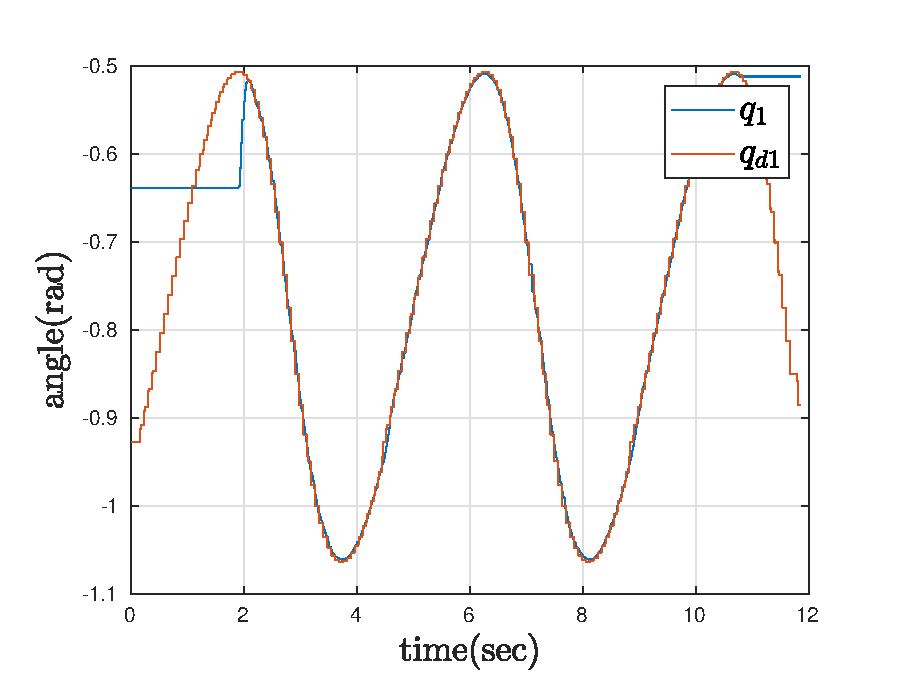
\includegraphics[width = \picsSiz\linewidth]{img/pathF1ff.eps}
        \caption{ }
    \end{subfigure}
    ~ 
    \begin{subfigure}[htbp]{0.45\textwidth}
        \centering
        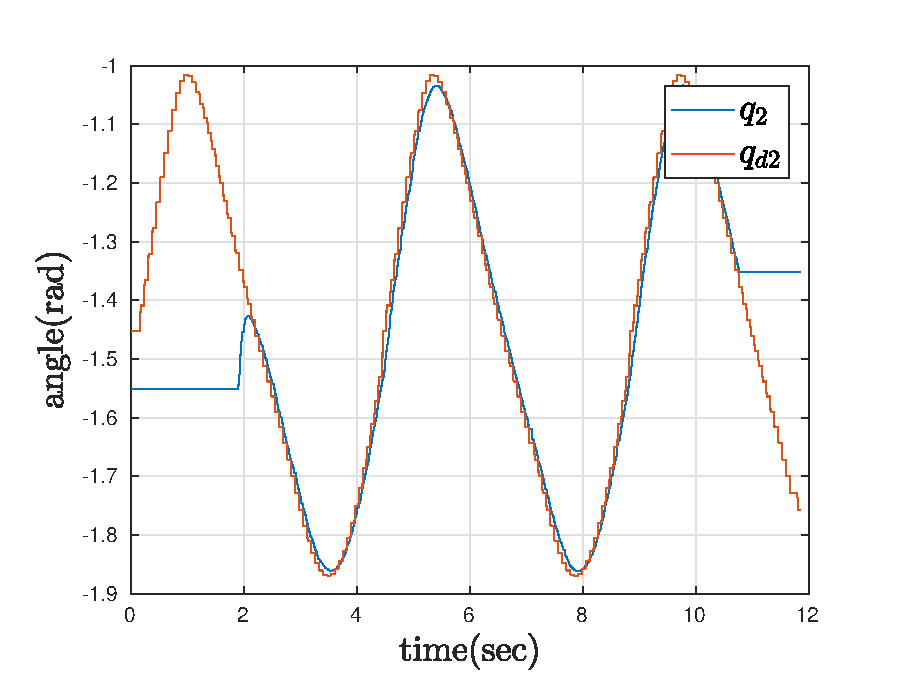
\includegraphics[width = \picsSiz\linewidth]{img/pathF2ff.eps}
        \caption{ }
    \end{subfigure}
    ~
    \centering
    \begin{subfigure}[htbp]{0.45\textwidth}
        \centering
        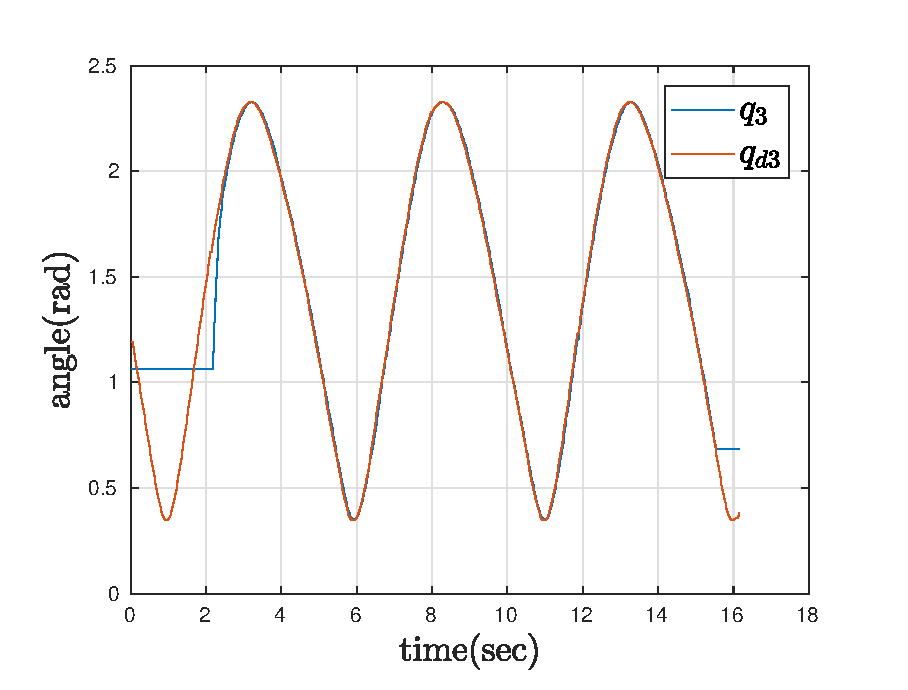
\includegraphics[width = \picsSiz\linewidth]{img/pathF3ff.eps}
        \caption{ }
    \end{subfigure}
    ~ 
    \begin{subfigure}[htbp]{0.45\textwidth}
        \centering
        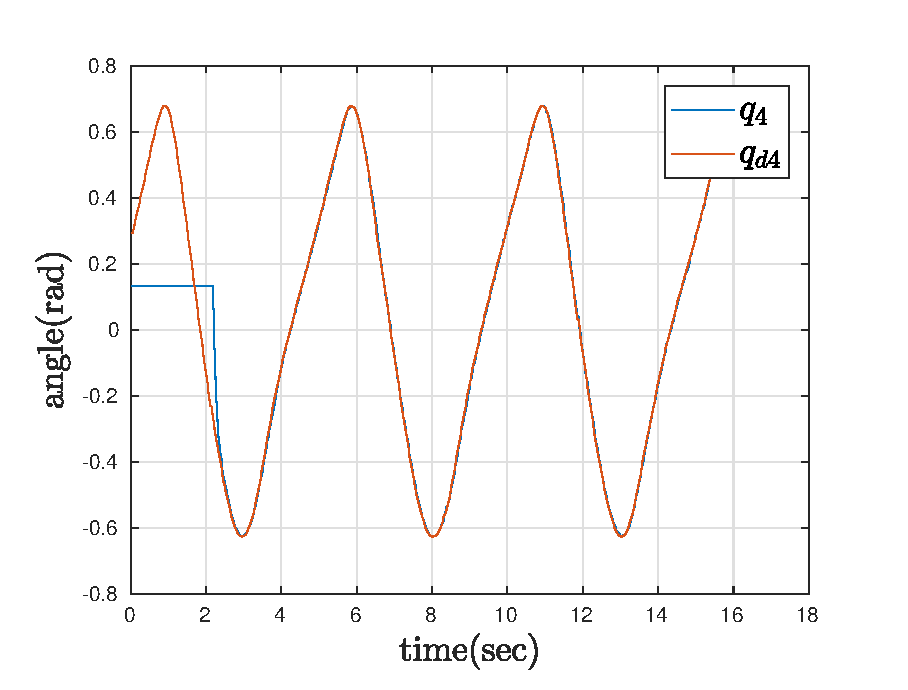
\includegraphics[width = \picsSiz\linewidth]{img/pathF4ff.eps}
        \caption{ }
    \end{subfigure}
    ~
    \begin{subfigure}[htbp]{0.45\textwidth}
        \centering
        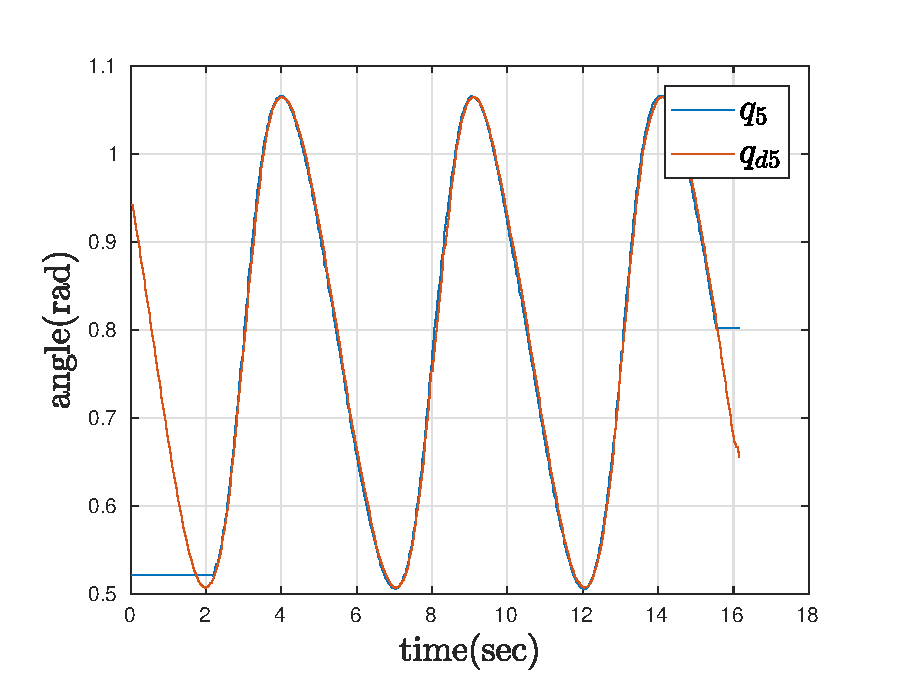
\includegraphics[width = \picsSiz\linewidth]{img/pathF5ff.eps}
        \caption{ }
    \end{subfigure}
    \caption{Path following with with more set points}
    \label{fig:pathTSff}
\end{figure*}



\clearpage
\section{Trajectory planning}
\subsection{Point to point tracking}
The manipulator is most likely to follow a path so it is desirable to test the controller for a path as well. The \figref{fig:pathTS} shows how each joint manages to follow the desired path used in Chapter \ref{chap:kinematics} shown in \figref{fig:IKcom} . One can see that the robot lags behind the desired path. This path is only time dependent so it changes without respect to if the robot arm has managed to get the desired position or not.\\\\
\def\picsSiz{1.08}
\begin{figure*}[htbp]
    \centering
    \begin{subfigure}[htbp]{0.45\textwidth}
        \centering
        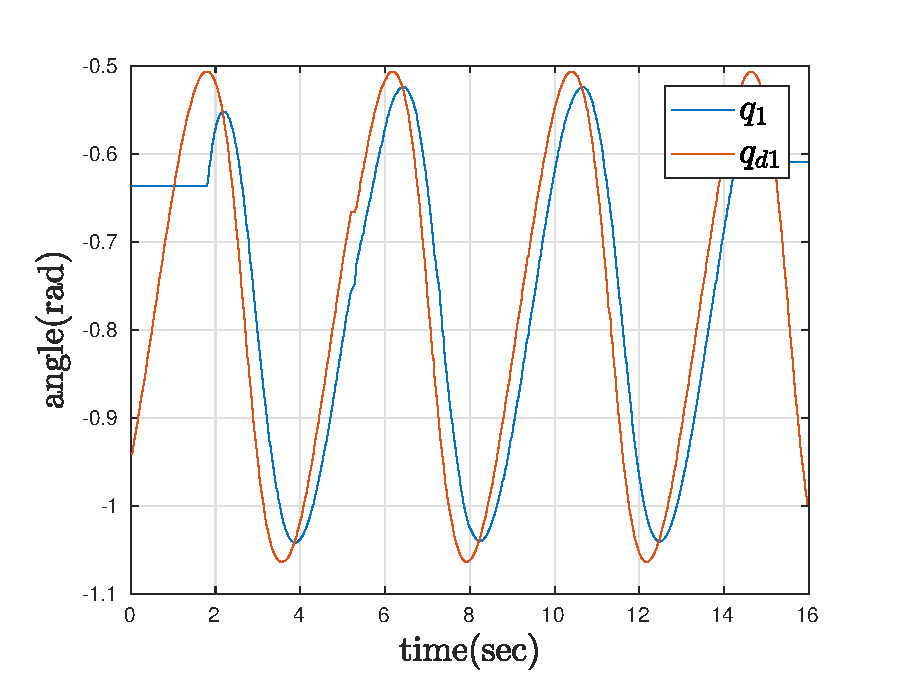
\includegraphics[width = \picsSiz\linewidth]{img/pathF1.eps}
        \caption{}
    \end{subfigure}
    ~ 
    \begin{subfigure}[htbp]{0.45\textwidth}
        \centering
        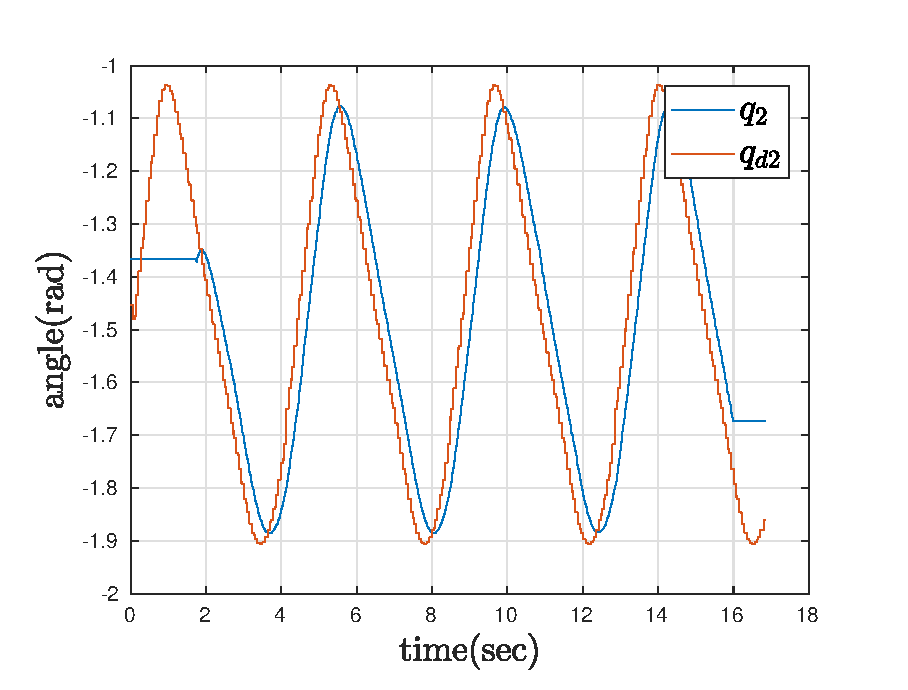
\includegraphics[width = \picsSiz\linewidth]{img/pathF2.eps}
        \caption{}
    \end{subfigure}
    ~
    \centering
    \begin{subfigure}[htbp]{0.45\textwidth}
        \centering
        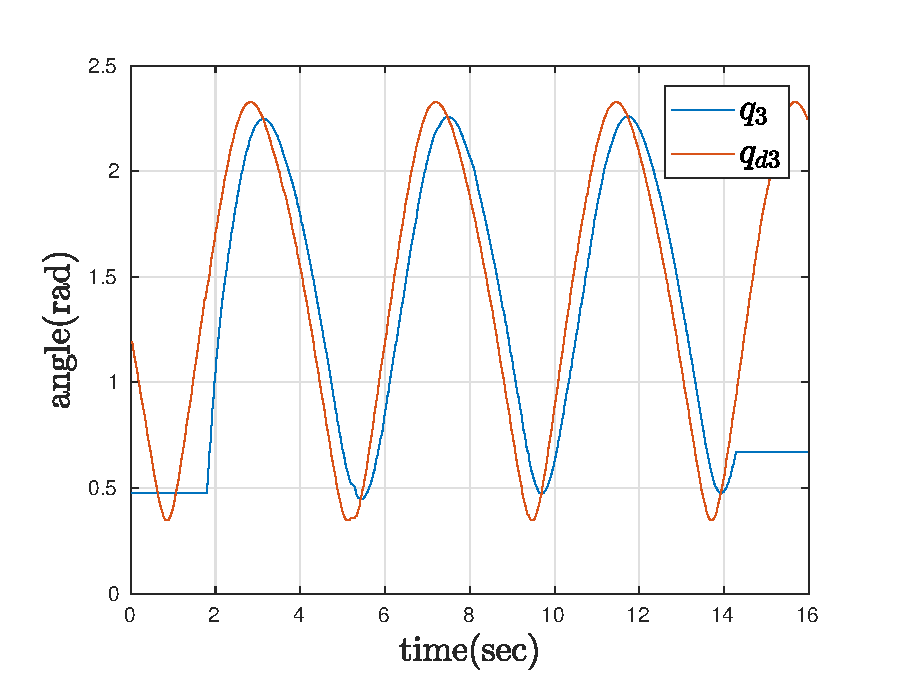
\includegraphics[width = \picsSiz\linewidth]{img/pathF3.eps}
        \caption{}
    \end{subfigure}
    ~ 
    \begin{subfigure}[htbp]{0.45\textwidth}
        \centering
        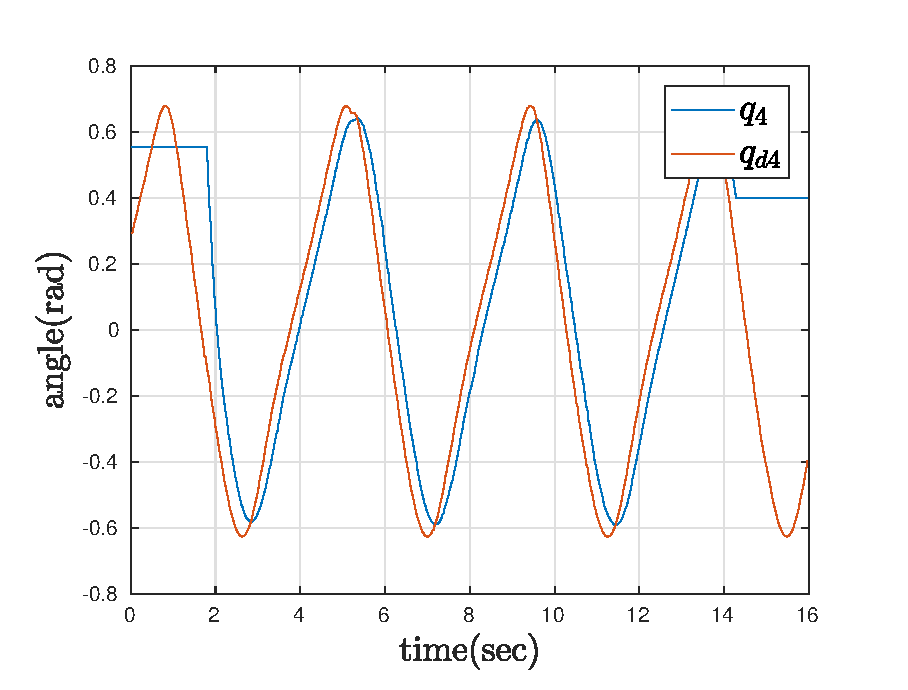
\includegraphics[width = \picsSiz\linewidth]{img/pathF4.eps}
        \caption{}
    \end{subfigure}
    ~
    \begin{subfigure}[htbp]{0.45\textwidth}
        \centering
        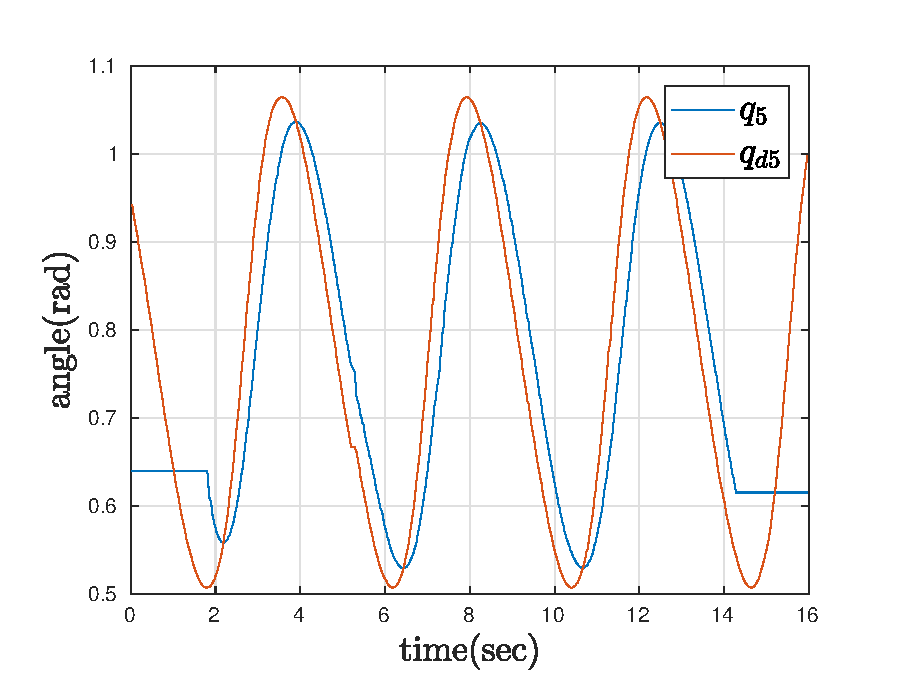
\includegraphics[width = \picsSiz\linewidth]{img/pathF5.eps}
        \caption{}
    \end{subfigure}
    \caption{Path following}
    \label{fig:pathTS}
\end{figure*}
The only information the robot gets is the point it is supposed to get to and it changes before it can reach it. It is therefore wanted to pass it some more information about the path. Reference \cite{Siciliano} gives a method to use the slope of the trajectory to find the joint velocity in the trajectory:
\begin{align*}
    \dot{q}_{d_i} = 
    \begin{cases}
    0\hphantom{ \frac{1}{2}(v_i+v_{i+1})}\;\;sgn(v_k)\ne sgn(v_{i+1})\\
    \frac{1}{2}(v_i+v_{i+1}) \quad  sgn(v_i)= sgn(v_{i+1})
    \end{cases}
\end{align*}
where $v_i = \frac{q_i-q_{i-1}}{t_i-t_{i-1}}$ and when the last point $N$ is reached, the joint velocity $q_N$ should be zero. Since the error between the executed trajectory and the desired trajectory can be seen as a time delay one can also add the next points as a reference:
\begin{align*}
    \tilde{q} = q_{d_i}-q + \frac{q_{d_{i+1}}-q }{2}+\frac{q_{d_{i+2}}-q }{2}
\end{align*}
The results are given in \figref{fig:pathTSff}. One can see that the error is almost gone. The reason integral action is not used here is because integral action is best when dealing with steady state constant errors which is not the case here\footnote{The gravity component in the controller acts as integral action by cancelling the gravity forces influencing the manipulator}. Integral action will also include more oscillations and instability to the system which is undesirable.



\def\picsSiz{1.08}
\begin{figure*}[htbp]
    \centering
    \begin{subfigure}[htbp]{0.45\textwidth}
        \centering
        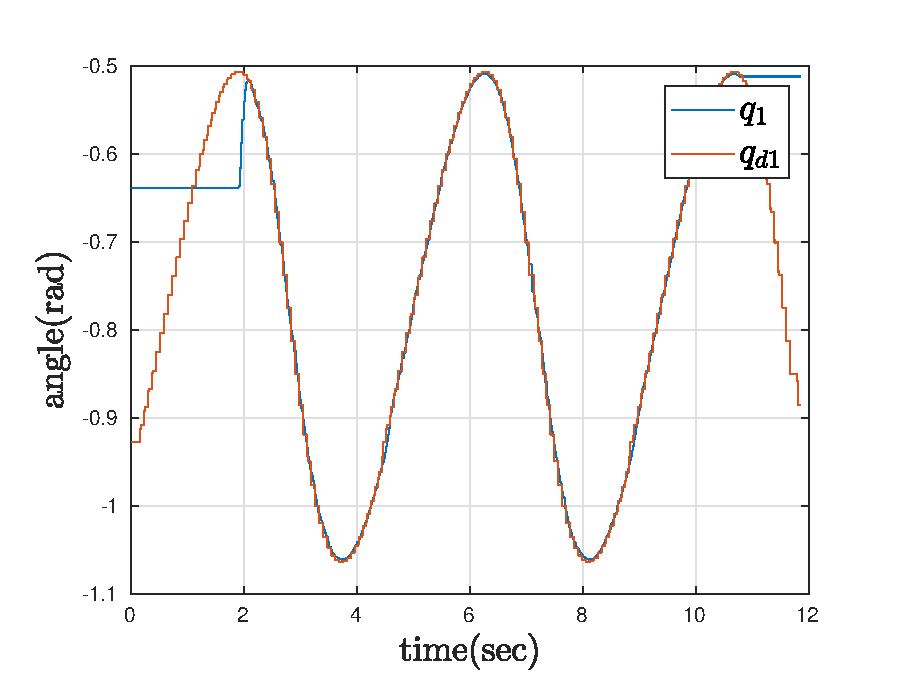
\includegraphics[width = \picsSiz\linewidth]{img/pathF1ff.eps}
        \caption{ }
    \end{subfigure}
    ~ 
    \begin{subfigure}[htbp]{0.45\textwidth}
        \centering
        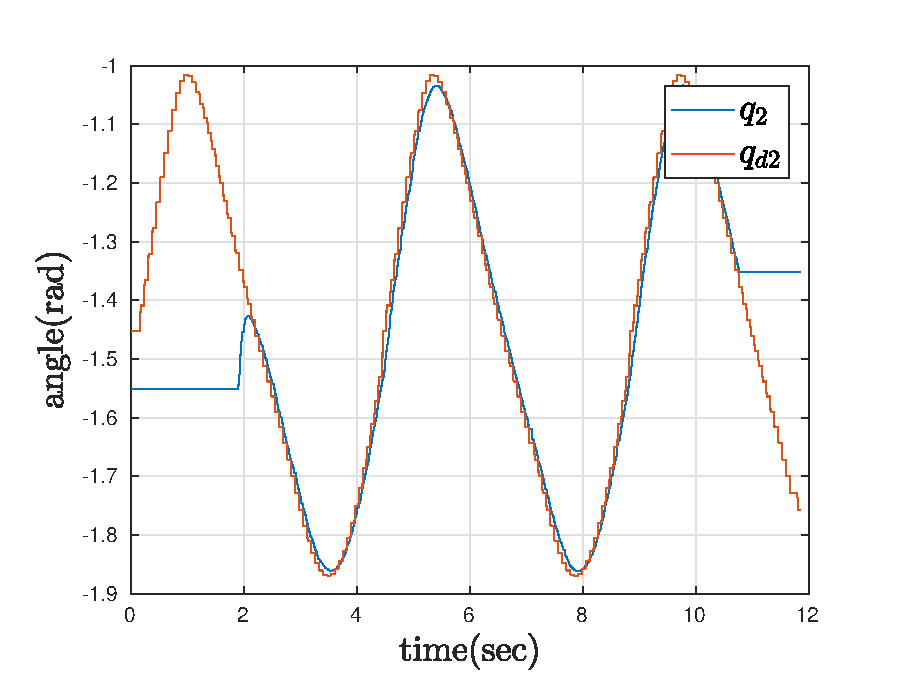
\includegraphics[width = \picsSiz\linewidth]{img/pathF2ff.eps}
        \caption{ }
    \end{subfigure}
    ~
    \centering
    \begin{subfigure}[htbp]{0.45\textwidth}
        \centering
        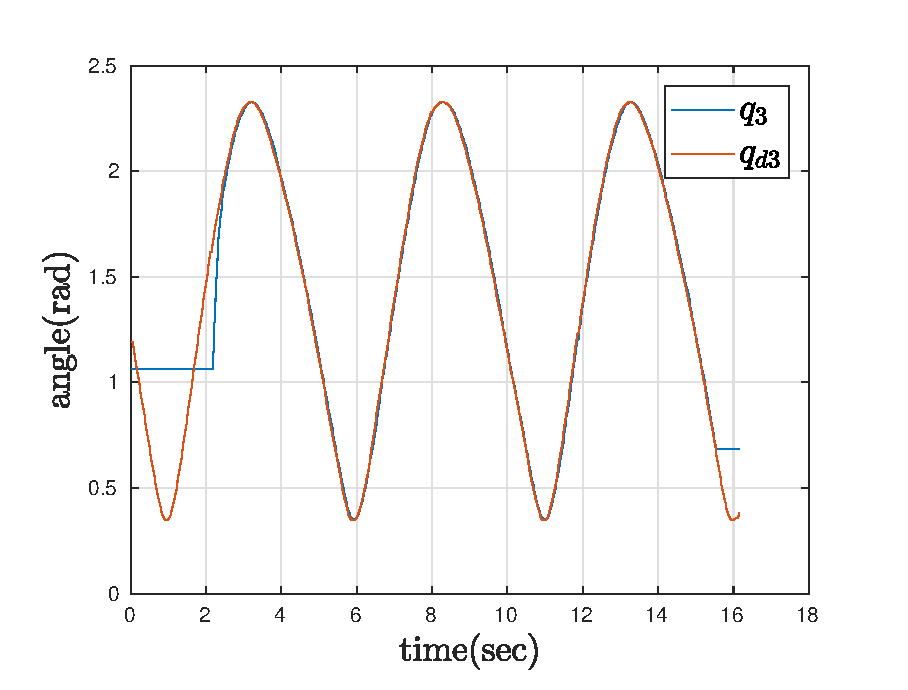
\includegraphics[width = \picsSiz\linewidth]{img/pathF3ff.eps}
        \caption{ }
    \end{subfigure}
    ~ 
    \begin{subfigure}[htbp]{0.45\textwidth}
        \centering
        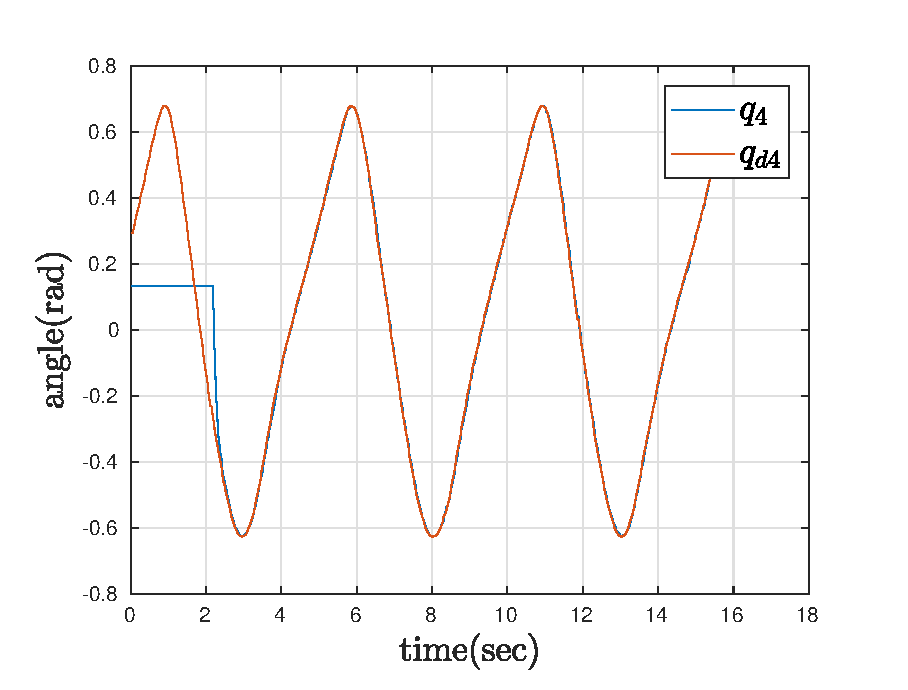
\includegraphics[width = \picsSiz\linewidth]{img/pathF4ff.eps}
        \caption{ }
    \end{subfigure}
    ~
    \begin{subfigure}[htbp]{0.45\textwidth}
        \centering
        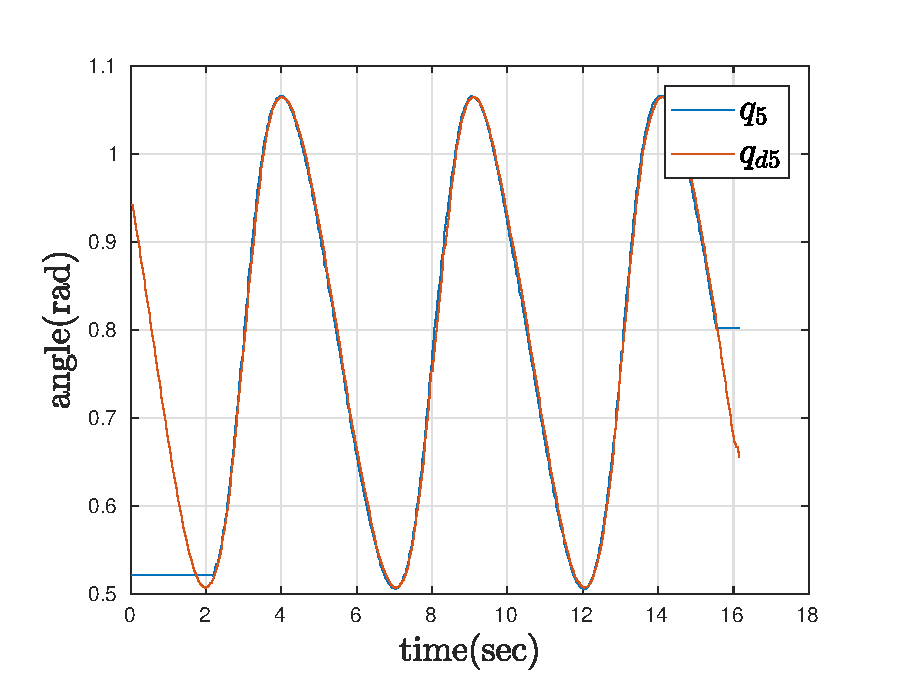
\includegraphics[width = \picsSiz\linewidth]{img/pathF5ff.eps}
        \caption{ }
    \end{subfigure}
    \caption{Path following with trajectory planner}
    \label{fig:pathTSff}
\end{figure*}
\newpage

\section{Motion planning}
Until now we have just used a predefined path that has been made to test the different aspects of the controller. If it is wanted to go from one point to another, it can be solved by creating a spline between these two points and do path following\cite{Spline,MatlabSpline2,MatlabSpline}. The task is not so easy if there are obstacles present. We then need to find the set-points such that the obstacle is avoided. One algorithm for solving this is the \textit{rapidly-exploring random tree (RRT)} which gives good results without any parameter tuning\cite{Lavalle}. 

\subsection{Rapidly exploring Random Tree (RRT)}
The RRT algorithm is creating a space-filling tree. In our case it can be used with obstacles in the search space such that the obstacle will be an illegal object where the three cannot expand. Then the shortest path is used to find a path trough the tree such that we get to the desired point and avoiding the obstacle. In \autoref{alg:rdt} one can see the \textit{simple rapidly exploring dense trees(RDT)} algorithm presented by \cite{Lavalle}. The difference between RRT and RDT is that the RDT is using a dense sequence $\alpha(i)$, and for RRT $\alpha(i)$ is a random value. This algorithm is without obstacle avoidance. If obstacle avoidance is wanted one have to check that the new edge does not intersect the obstacle. %If it intersects one have to find another vertex.\\\\
\begin{algorithm}[htbp]
 %\KwData{this text}
 %\KwResult{how to write algorithm with \LaTeX2e }
 SIMPLE\_RDT($q_0$)\;
 $\mathcal{G}.init(q_0)$\;
 \For{$i=1$ to $k$}{
  $\mathcal{G}.add\_vertex(\alpha(i))$\;
  $q_n\longleftarrow NEAREST(S(\mathcal{G}),\alpha(i))$\;
  $\mathcal{G}.add\_edge(q_n,\alpha(i))$\;
 }
 \caption{RDT algorithm}
 \label{alg:rdt}
\end{algorithm}

Reference \cite{rrt} provides code to find a path using RRT. In \figref{fig:rrt2dex} an example is given of the algorithm. An obstacle has been placed in the search space and the wanted point is behind the obstacle relative to the start point which in this case is the origin \cite{rrt}.
\begin{figure}[htbp]
  \centering
  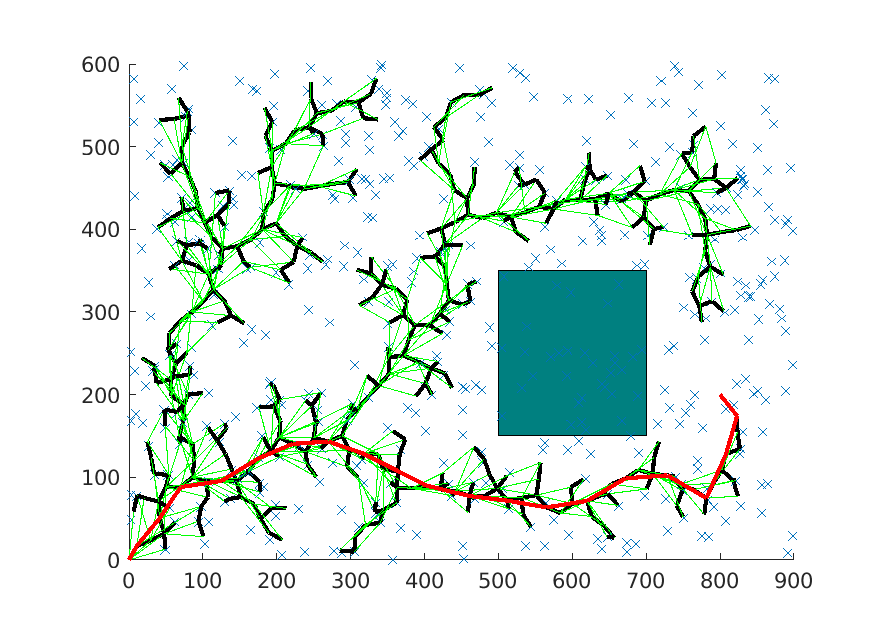
\includegraphics[width=.9\textwidth]{img/rrt2dex.eps}
  \caption{2D example of the RRT algoritm}
  \label{fig:rrt2dex}
\end{figure}

The next step is to expand this to a 3D example and do the same there. The code provided by \cite{rrt} does include 3D RRT, but not with obstacle avoidance unfortunately. But the source code is given, which mean it can be augmented into covering 3D obstacle avoidance. In \figref{fig:rrt3dex} the result of RRT in 3D space is presented. The red line is the lines between the nodes in the tree which shows a path to the desired point. 
\def\picsSiz{1.08}
\begin{figure*}[htbp]
    \centering
    \begin{subfigure}[htbp]{0.45\textwidth}
        \centering
        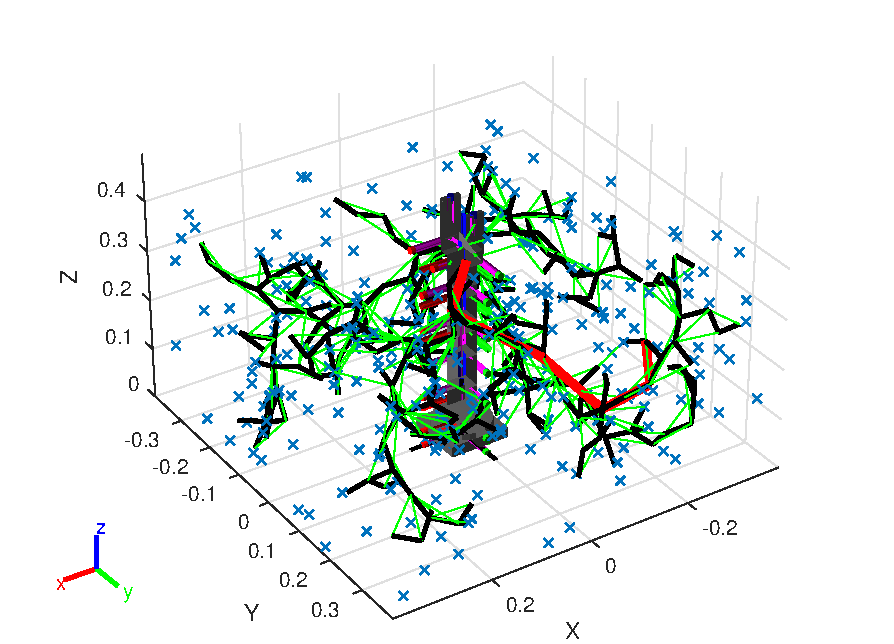
\includegraphics[width = \picsSiz\linewidth]{img/rrt3dex.eps}
        \caption{Result of the RRT algorithm}
        \label{fig:rrt3dex}
    \end{subfigure}
    ~ 
    \begin{subfigure}[htbp]{0.45\textwidth}
        \centering
        \includegraphics[width = \picsSiz\linewidth]{img/rrtSpline.eps}
        \caption{A spline is found based on the results}
        \label{fig:rrtSpline}
    \end{subfigure}
    \caption{3D example of the RRT algoritm}
    \label{fig:rrtsuper}
\end{figure*}
 As one can see in \figref{fig:rrt3dex} there are some green lines. These lines can be seen as shortcuts between each node the length of these shortcuts can be changed. In \figref{fig:rrtSpline} we have a path that is more complicated than it should be and one should maybe consider to increase the length of the shortcuts to get less nodes. This means that if the shortcut length is big enough the path will be a straight line from the desired point to the starting point of the tree. Given that the tree has found a path to the point. 
 
 \subsubsection{Obstacle avoidance}
 There is no point in doing the RRT if one does not have an obstacle to avoid. When an obstacle is added to the searchspace one have to check if the line connecting the new node to its parent node does not intersect with the object. The same has to be done with the shortcuts. To check if the edgdes and lines intersects with the obstacle Smits algorithm for ray intersection with a box is used\cite{Smits,Intersection}. In \figref{fig:obav} one can see the results when an obstacle is added into the workspace. The RRT algorithm finds as decent path and a spline is generated based on the results. 

\def\picsSiz{1.08}
\begin{figure*}[htbp]
    \centering
    \begin{subfigure}[htbp]{0.45\textwidth}
        \centering
        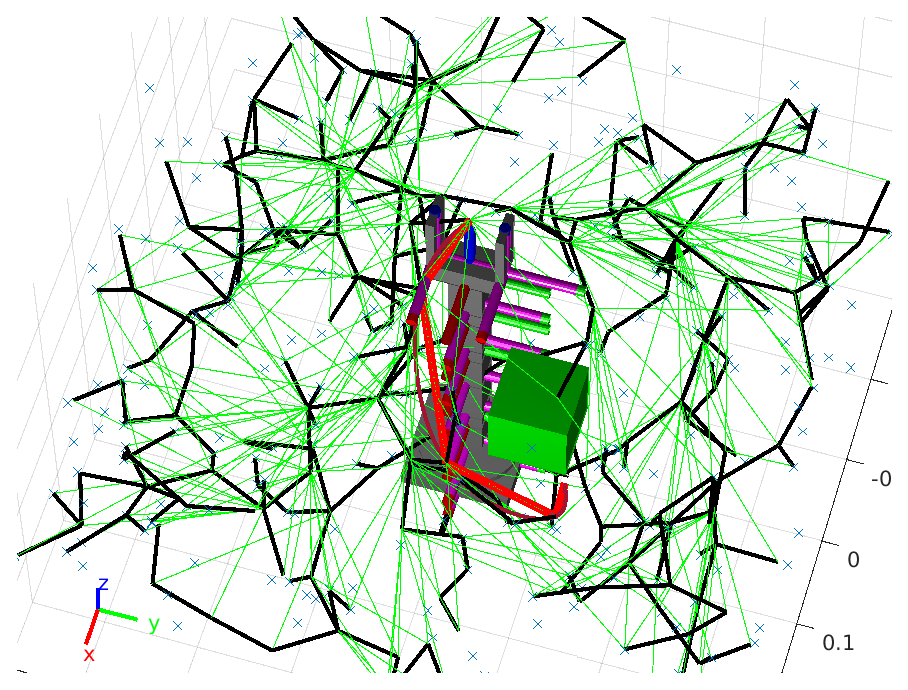
\includegraphics[width = \picsSiz\linewidth]{img/rrt3dOBav.eps}
        \caption{Result of the RRT algorithm with an obstacle}
        \label{fig:obav1}
    \end{subfigure}
    ~ 
    \begin{subfigure}[htbp]{0.45\textwidth}
        \centering
        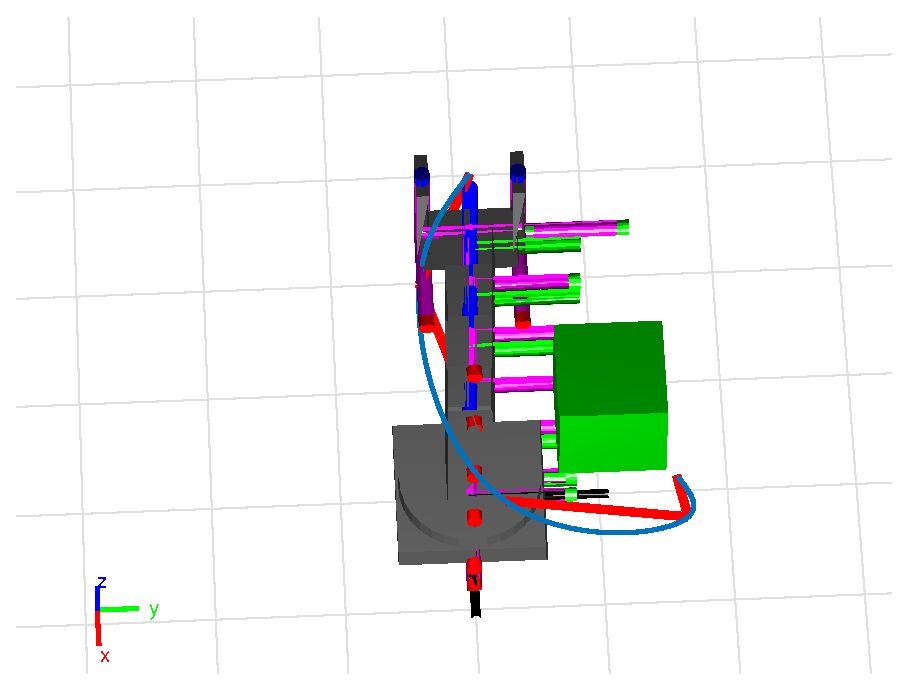
\includegraphics[width = \picsSiz\linewidth]{img/rrt3dOBavPath.eps}
        \caption{A spline is found based on the results}
        \label{fig:obav2}
    \end{subfigure}
    \caption{3D example of the RRT algoritm with obstacle present}
    \label{fig:obav}
\end{figure*}

\chapter{Conclusion}
In this project several aspects of robotics have been considered. The first topic is visualization and simulation where a virtual model of a given robot is made. This includes measurements, mass and moments of inertia. Some of the measurements and mass is only guessed or estimated and it may not result in a perfect recreation of the actual robot. The moments of inertia are also found based on simplifications and if one want a more realistic behaviour of the robot it may be by recalculating this. The simulation environment Gazebo is a good software with much support online in forums and wikis. There was however some trouble when implementing the moments of inertia that would lead to the robot not spawning properly, because of too low inertia of the two fingers.\\\\
The second part that was presented was the kinematics problem where the forward kinematics was found. The DH convention was used to find this. Then the inverse kinematics problem were solved by using the MATLAB robotics toolbox\cite{MatlabRobTool}. The toolbox gave good and precise solutions and was easy to use. One thing that may not be so good is that it uses about 100ms per set point which may be too slow for an online planner\cite{spong}, but if offline planning is the purpose the time consumption does not matter.
\\\\
The next part is the control and motion planning. The PD controller with gravity compensation is a basic controller which worked well for this case, but a better controller should be considered. Both \cite{spong} and \cite{Siciliano} are good resources when considering more advanced controllers. This project includes a way to plan a simple path with a single obstacle present in it. The trajectory is not found though, because of the obstacle one does not want only the end effector to avoid the obstacle, but the rest of the robot manipulator must avoid it as well which is a more complex problem and should be included in further work. In fact, the motion planning is a very complex task and \cite{spong} states that path and trajectory planning is one of the most difficult problems in computer science.


\backmatter
\addcontentsline{toc}{chapter}{\bibname}
\bibliography{bib/bibliography}


\end{document}
